%% *************************************************************************
%%                                                            raa.tex
%% RAA Ver. 1.0, LaTeX class for Research in Astronomy & Astrophysics
%% demonstration file
%%                      by Zhou Ai-Ying, since 2001.08.28
%%
%% Note: 1. Pay close attention to the format of RAA's reference list and
%%          other requirements. See Instructions for Authors at the web site:
%%          http://www.chjaa.org
%%       2. Final publication layout and web version will be produced with
%%          this LaTeX source file. Please write clean text.
%%---------------------------------------------------------------------------------
%%

\documentclass[referee]{raa}            % referee version: for submission
\usepackage{graphicx,times}
\usepackage{natbib}
\usepackage{amssymb,amsmath}
\bibpunct{(}{)}{;}{a}{}{,}


\usepackage[a4paper=true,dvipdfm=true,pagebackref=true]{hyperref}
% \hypersetup{pdftitle = The title of my PDF, pdfauthor = My name, pdfsubject= The subject, pdfkeywords = keyword1 keyword2 keyword3}
\hypersetup{colorlinks = true, linkcolor = green, anchorcolor = red, citecolor = blue, filecolor = red, pagecolor = red, urlcolor = red}

%% manuscript produces a one-column, double-spaced document
%\linespread{1.6}
\begin{document}

   \title{On the Construction of New Stellar  Classification Templates Library for LAMOST Spectra Analysis Pipeline
%\,$^*$
%\footnotetext{$*$ Supported by the National Natural Science Foundation of China.}
}
%   \subtitle{I. Place Your Subtitle Here}

   \volnopage{Vol.0 (200x) No.0, 000--000}      %%preserved for Editor. DOn't remove!
   \setcounter{page}{1}          %%starting page, preserved for Editor. DOn't remove!
   \author{
Peng Wei
      \inst{1,2}
   \and  Ali* Luo
      \inst{1,3}
\and  Yinbi Li
      \inst{1}
\and  Jingchang Pan
      \inst{3}
\and  Fengfei Wang
      \inst{1}
\and  Jiannan Zhang
      \inst{1}
          \and  Liangping Tu
       \inst{1,4}
       	\and  Bin Jiang
       \inst{3}
    \and  Yongheng Zhao
      \inst{1}
\and  Jianjun Chen
      \inst{1,2}
\and  Xiaoyan Chen
      \inst{1}
\and  Bing Du
      \inst{1}
\and  Wen Hou
      \inst{1,2}
\and  Ge Jin
 \inst{6}
 \and  Xiao Kong
      \inst{1,2}
    \and  Jie Liu
      \inst{3}
       	\and  Juanjuan Ren
       \inst{1,2}
 \and  Yihan Song
      \inst{1}
    \and  Yue Wu
      \inst{1}
       	\and  Haifeng Yang
       \inst{1,2,5}
    \and  Zhenping Yi
      \inst{1,2,3}
}
%% Here is an example of three authors come from different institutes.
%% For single author or all the authors from an institute, use "\inst{}" only
   \institute{
    Key Laboratory of Optical Astronomy,National Astronomical Observatories,  Chinese Academy of Sciences, Beijing, 100012, China
      {\it lal@nao.cas.cn weipeng@nao.cas.cn}\\
	  \and
    University of Chinese Academy of Sciences, Beijing, 100049, China\\
 	   \and
    School of Mechanical, Electrical and Information Engineering, Shandong University,Weihai, 264209, China\\
       \and
   School of Science, Liaoning University of Science and Technology,  Anshan, 144051, China
\and
School of Computer Science and Technology, Taiyuan University of Science and Technology,Taiyuan 030024, China
\and
University of Science and Technology of China, Hefei 230026, China
% % Please give the E-mail address of the author, to whom future correspondence and
% offprint requests will be sent.
   }

   \date{Received~~2009 month day; accepted~~2009~~month day}

\abstract{
The LAMOST spectra analysis pipeline is one of LAMOST softwares to produce and analyze the final spectra
and its aim is to classify and measure the spectra observed in the survey.
Through the pipeline, the observed stellar spectra are classified into different sub-classes by matching with templates spectra.
Consequently, the performance of the stellar classification is greatly influenced by the quality of templates.
%This paper presents the construction of the new stellar classification templates library for the LAMOST Spectra Analysis Pipeline.
A new LAMOST stellar spectral classification templates library is constructed, which is supposed to  improve the precision  and credibility  of the stellar classification.
About one million spectra are selected from LAMOST Data Release one (DR1) to construct the new stellar templates,
and they are gathered in 233 groups by two criteria:
I) pseudo g-r colors obtained by convolving the spectra  with the SDSS \emph{ugriz} filter response curve\
II) the subclass given by the pipeline.
%Meanwhile, some special types of spectra are manually picked out to add into the corresponding groups.
%In each group, some outliers are excluded, the Principal Component Analysis(PCA) method is applied to  the remaining  spectra,
%and all spectra are reconstructed using the first a few principal components.
%Finally, the weighted average spectra are constructed as the template spectra in the groups.
In each group, the template spectra are constructed within three steps:
I) Outliers are excluded using Local Outlier Probabilities (LoOP) algorithnm, and then the Principal Component Analysis(PCA) method is applied to  the remaining  spectra of each group.
About 5\% outliers are ruled out from one million spectra.
II) All remaining spectrum are reconstructed using by the first principal components of each group.
III) The weighted average spectra are made as the template spectra in the groups.
And we initially obtain  stellar tempalte spectra in 216 groups.
All template spectra are visually inspected, and 52 spectra are abadoned due to low spectral quality.
Furthermore, the MK classification for each template spectrum is manually determined by comparing with three libraries of label-known templates with known MK class.
Meanwhile, some unlabeled or wrongly labeled spectra are relabeled  or abandoned.
And we finally obtain 164 new template spectra with 65 different MK classes.
The template library is composed by the spectra left and the first version contains 164 spectra and 65 different MK classes.
\keywords{methods: data analysis, methods: statistical, surveys}
}

   \authorrunning{Wei Peng, Luo Ali et al. }            %author_head in even pages
   \titlerunning{On the Construction of Stellar  Classification Templates Library for LAMOST 1D Pipeline }  % title_head in odd pages

   \maketitle
%% The author head (on even pages) and the title head (on odd pages) will be
%% automatically extracted from \author{} and \title{}. Whenever the title is too long,
%% you will be asked to supply a shorter one by inserting either \authorrunning{} or
%% \titlerunning{} before \maketitle. Anyway, you can specify your own heads.
%%
%%
%% Note: In the following text body of your manuscript, please note several differences from
%%       other major journals:
%% (1) \subsection{Please Capitalize the First Letter of Each Notional Word in Subsection Title}
%% (2) Please Capitalize the First Letter of Each Notional Word in all tables' captions

%
%________________________________________________ sections below
%


\section{Introduction}           %% first-level sections will be auto-capitalized
\label{sect:intro}
The Large Sky Area Multi-Object Fiber Spectroscopic Telescope ��LAMOST�� is a special reflecting Schmidt telescope with an effective aperture of 3.6-4.9 m, a focal length of 20 m and a field of view (FOV) of 5$^\circ$ \citep{cui2012large}.
In virtue of its unique design, LAMOST can  observe  4000 spectra simultaneously in a single exposure.
Consequently, the LAMOST  has a great potential to efficiently survey a large volume of space for stars and galaxies.
%The LAMOST survey\citep{zhao2012lamost} contains two main parts: the LAMOST ExtraGAlactic Survey (LEGAS) and the LAMOST Experiment for Galactic Understanding and Exploration survey of Milky Way stellar structure(LEGUE, see \citet{deng2012lamost}).

The LAMOST data are processed by data processing softwares written specifically for the LAMOST Spectral Survey.
The LAMOST spectra analysis pipeline (also called 1D pipeline) \citep{luo2001steps,luo2004design,luo2008automated,wang2010calibration,luo2012data} is one of these softwares to produce and analyze final spectra.
%The pipeline is based on the specBS pipeline\citep{aihara2011eighth} for the analysis of SDSS spectra.
The pipeline performs  $\chi^2$ fits of the spectra to templates in wavelength space,
fitting spectra with linear combinations of eigen-spectra and low-order polynomials.
Through the pipeline, the observed stellar spectra are classified into different sub-classes.
Consequently, the performance of the stellar classification greatly depends on the quality of templates.


Considering the similiarity of  the LAMOST stellar spectra with other survey spectra,
some  spectra  selected from SDSS and MILES \citep{falcon2011updated} are used as templates for stellar classification in current LAMOST spectra analysis pipeline .
The current library contains 36 stellar subclasses plus 20 subclasses specially for A-type star.
The former 36 templates are constructed from a set of SDSS spectra \citep{wang2010calibration}.
while the latter 20 A-type template spectra are picked out  from MILES library .
These template spectra cover nearly all common types of stellar spectra in the survey.
Matching with these templates, the LAMOST stellar spectra are classified as different stellar sub-classes.
Although the majority of the LAMOST stellar spectra are correctly classified using current library,
there are some significant  differences between these spectra.
Firstly, the LAMOST , SDSS and MILES spectra have different resolutoins, 1800 , 2000 and 2000 respectively.
Secondly, different instrumental designs bring about differnt effects on the spectra.
In addition, the processes of spectrum extraction, wavelength calribration and flux calribration \citep{bai2012lamost} are also different.
Considering these issues which can not be ignored, it is very necessary to construct a new template library based on the  spectra  observed and processed by LAMOST.


In this paper, we described  in detail the construction of the new LAMOST stellar  classification template library.
The paper is organized as follows:
Section \ref{sect:construction} detailedly describe the construction process of the LAMOST stellar template library.
%Section \ref{sect:construction}
%Section \ref{sect:Sample} describes the used spectra from LAMOST Data Release One (DR1).
%The detailed description of used spectra from LAMOST, the template library construction steps, the related methods and the group dividing are outlined in section \ref{sect:construction}.
The results and discussions are given in section \ref{sect:Results}.
A brief summary is given in section \ref{sect:Summary}.
\section{The construction of the templates library}
\label{sect:construction}
\subsection{The Spectra From LAMOST Data Release One (DR1)}
%\label{sect:Sample}
The first data release (DR1) of LAMOST survey contains the spectra in the pilot survey and the first year of general survey.
The pilot survey of LAMOST  was launched on Oct 2011 , and ended on June 2012.% and about 31,900 spectra were released \citep{luo2012data}.
The first year of the LAMOST regular survey began from September 2012 and ended on June 2013.
The DR1 totally contains 2,204,860 spectra, including 717,660 spectra of pilot survey and 1,487,200 spectra of regular survey.
The sky coverage of LAMOST DR1 is shown in Fig \ref{Fig_all}.
 \begin{figure}
   \centering
   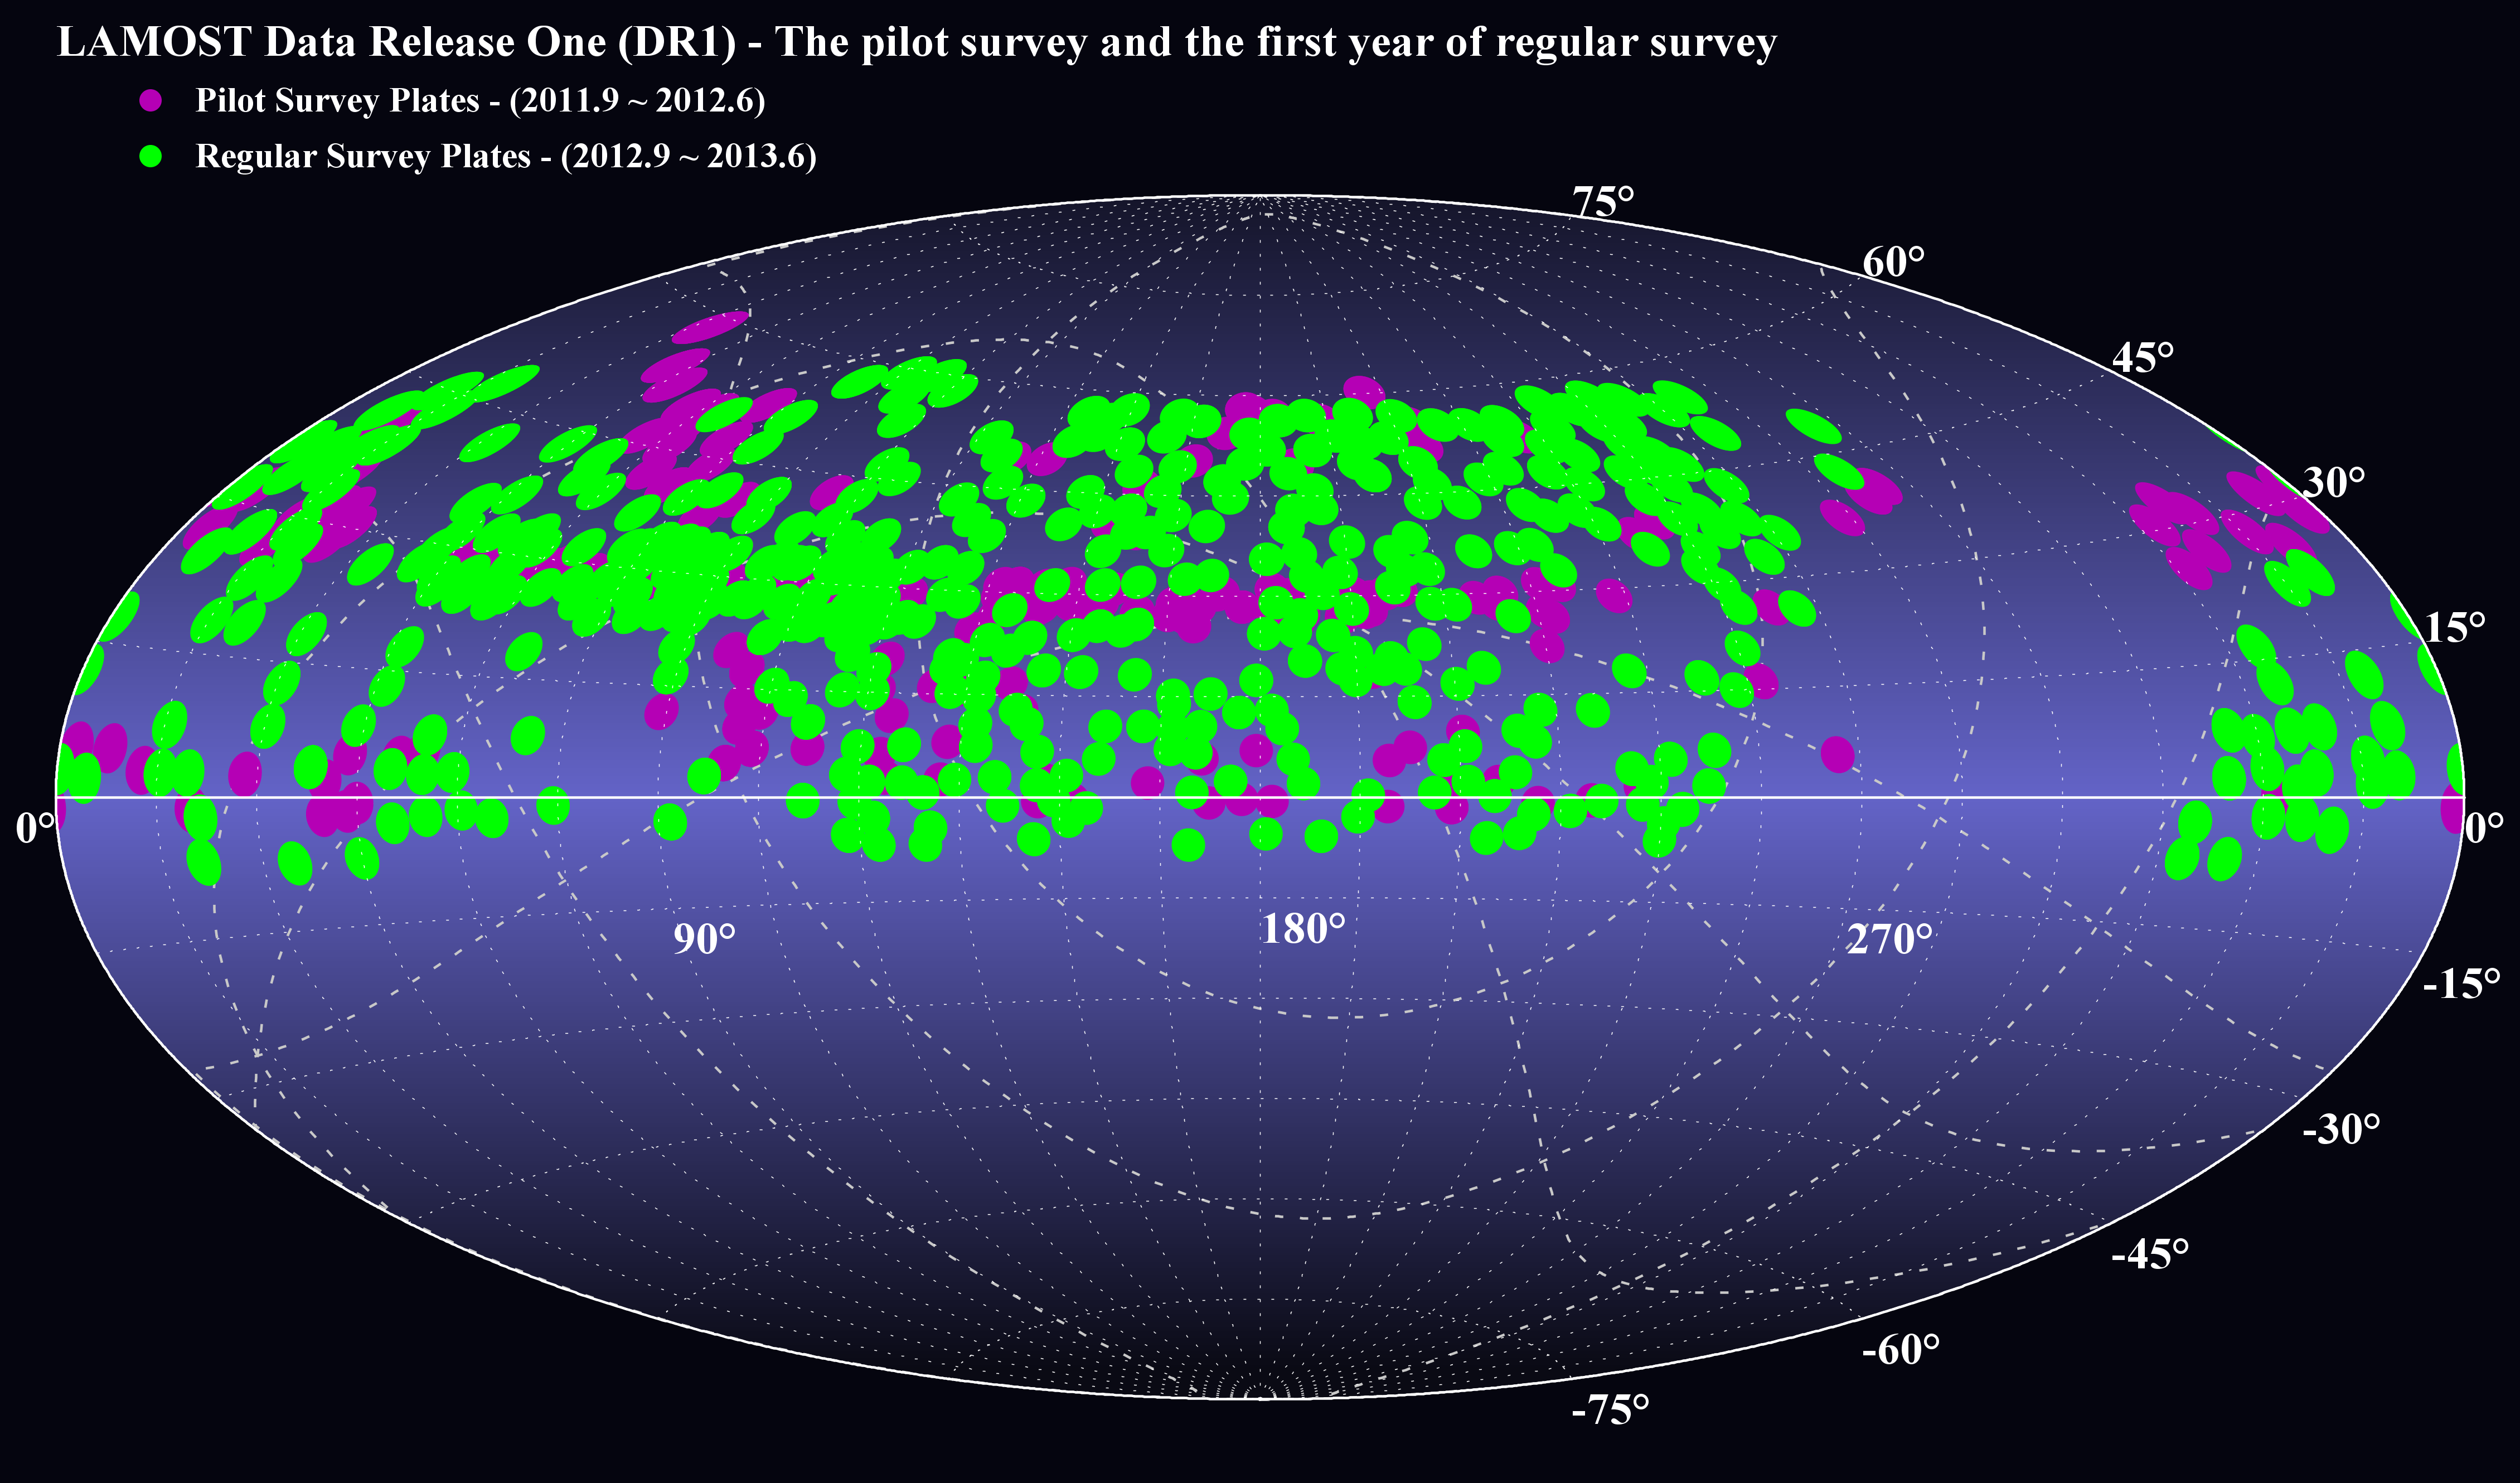
\includegraphics[width=14cm, angle=0]{dr1-full.eps}
   \caption{The LAMOST DR1  skycoverage  (\url{http://data.lamost.org/u/img/dr1-full.png}
   }
   \label{Fig_all}
   \end{figure}
%In addition, the atmospheric parameters of 1,085,404 stars are calculated, which becomes the largest stellar spectral parameters catalog in the world at present.

%The LAMOST survey has obtained spectra of stars in the Milky Way,
%which includes fainter objects on dark nights  \citep{yang2012legue,carlin2012algorithm},
%brighter objects on bright night  \citep{zhang2012legue},
%objects in the disk of the Galaxy with low latitude  \citep{chen2012legue} and objects in the region of the Galactic Anti-Center \citep{liu2013lss}.

%For LAMOST spectra with low confidence in measurement or low SNR, human checking is also applied to data quality \citep{luo2012dr1}.
%To publish relatively high quality spectra from all the data,  319 000 spectra are left as the released data following the rule proposed in  \cite{luo2012data}.
There are totally 1,946,429 stellar spectra in LAMOST DR1 and 1,173,928 spectra with SNR$>$10.
The spectral resolution R is about 1800 around g band with a 2/3 silt width  \citep{wang2013effects} and the wavelength coverage is from 3700 \AA\  to 9100 \AA.
%Two arms of each spectrograph covers the wavelength range and overlaps in 200\AA.
 %The spectra in the pilot survey go through the same data processing pipeline as the regular survey.
To extract spectra from raw observation data, the raw data have been reduced with LAMOST 2D pipeline \citep{bai2012lamost} including bias subtraction, cosmic-ray removal, spectral trace and extraction, flat-fielding, wavelength calibration sky subtraction, and combination.
%For the spectra with SNR$>$5
Then the 1D pipeline \citep{wang2010calibration,luo2012data} gives spectral type and redshift (radial velocity
 for stellar spectra).
Considering the  effect of interstellar dust  extinction on the spectra and the closeness of stars,
a mount of 855,583 spectra in the Galactic Anti Center and M31\citep{liu2013lss} whose plate name in the catalogue starts with 'GAC' or 'M31' are excluded.
And then  1,090,846 stellar spectra are left,
which are used for the construction of template library.

%In addition, some other spectra are  excluded in the construction of the library.%, which will be discussed in the section \ref{sect:construction}.
%  \cite{york2000sloan}
\subsection{Spectra Grouping}
We gather the left 1,090,846 spectra in 233 different groups to construct different kinds of templates,
by two criteria:
the proposed $g^*-r^*$ color and the subclass labeled by the pipeline.

\subsubsection{The pseudo g-r color}
%  \cite{mcgurk2010principal} divided all selected SDSS stellar spectra into different bins by the color g-r.
LAMOST is a spectroscopic survey oriented telescope and its photometric data are from different catalogs of other surveys.
Meanwhile, the flux calibration of LAMOST spectra is relative \citep{bai2012lamost}.
Therefore, accurate and uniform  colors can not be obtained for LAMOST spectra.
Inorder to slove this problem, we propose a pseudo g-r color(hereafter g$^*$-r$^*$) obtained by convolving each observed spectra with the SDSS $ugriz$ filter response curves.
The calculation method is described in detail  as follows:
\begin{enumerate}
 \item Suppose that the sampling points of   $g$ and $r$ filter response curves are $P_g$, $P_r$ respectively , and the response values are $C_g$, $C_r$.
 \item Interpolate the  flux of the observed spectra in the points of $P_g$ and $P_r$  to get $F_g$ and $F_r$.
 \item Get the pseudo color $g^*$-$r^*$:
 \begin{equation}
        g^*-r^*=-2.5*log\frac{F_g\bigotimes C_g}{\sum C_g} +2.5*log\frac{ F_r\bigotimes C_r}{\sum C_r}
       \end{equation}
\end{enumerate}


The g-r color  is a very good indicator of stellar surface effective temperature (Teff) \citep{lee2008segue,ivezic2008milky},
so we select objects with SDSS $ugriz$ magnitudes and signal to noise ratio (SNR) larger than 20 to check  whether
the relationship between the $g^*-r^*$ and the Teff exists.
The average value and standard deviation of $g^*$-$r^*$ for different spectral types (O, B, A, F, G, K, M-type) are calculated.
And as shown in Figure \ref{Fig1}, the $g^*$-$r^*$ color varies obviously for each spectral type.
 %we can infer that our defined $g^*-r*$ color can also be a good indicator of effective temperature.
 \begin{figure}
   \centering
   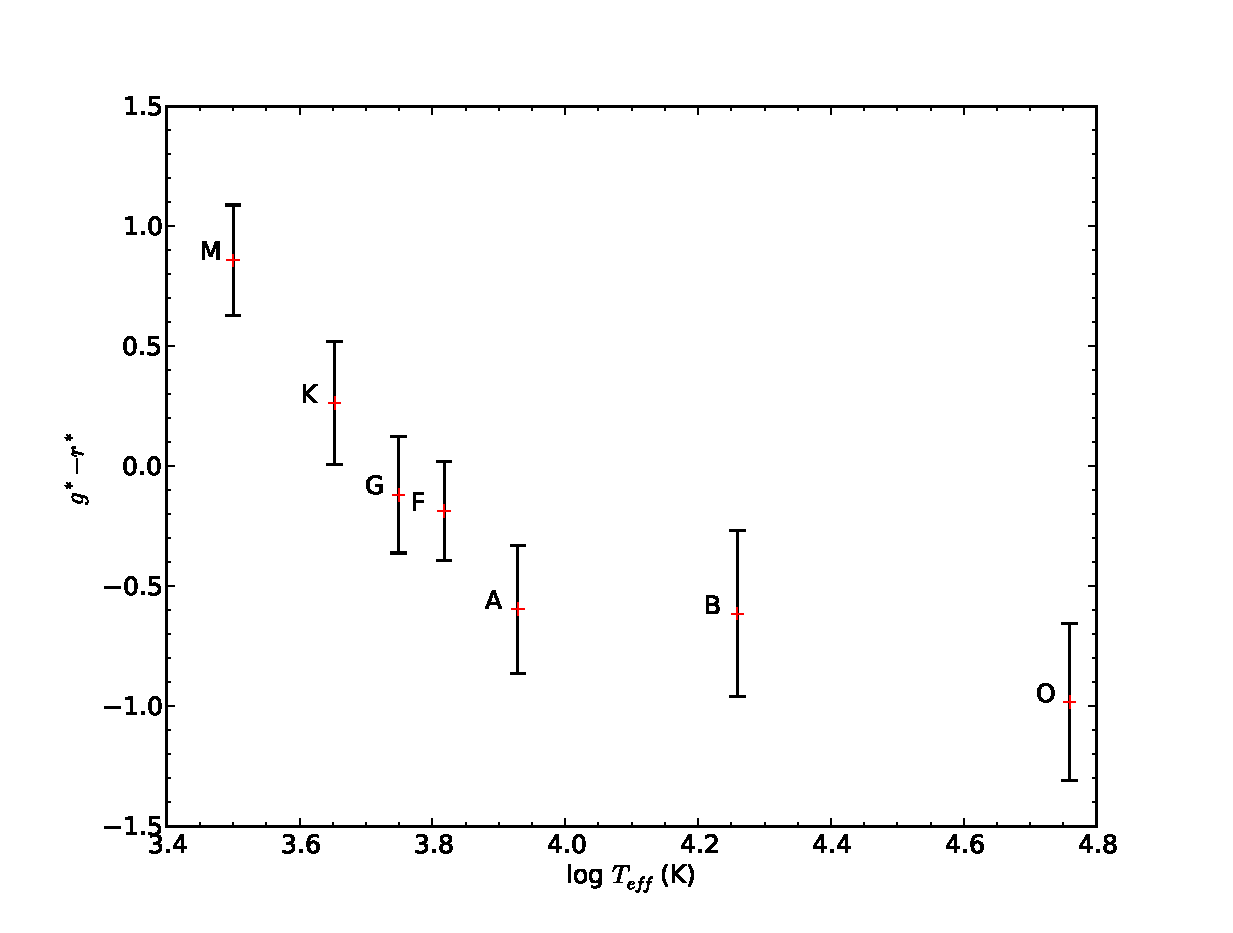
\includegraphics[width=10cm, angle=0,clip]{f5.eps}
   \caption{The average value and standard deviation of $g^*$-$r^*$ for  each spectral type.
    The X value of  the error bar is the median effective temperature in theory.
   The y value of the center of each error-bar is the average  $g^*$-$r^*$ color and the half length is the standard deviation of $g^*$-$r^*$.
   }
   \label{Fig1}
   \end{figure}

For these selected objects, the relationship between g-r color and $g^*$-$r^*$ is  shown in Fig.\ref{Fig2}.
There is a obvious linear relationship between the two colors,
and the derived best-fit expression is shown in formula \ref{eq2}:
\begin{equation}
 g-r=0.807* (g^*-r^*)+  0.655
 \label{eq2}
\end{equation}

 \begin{figure}
   \centering
   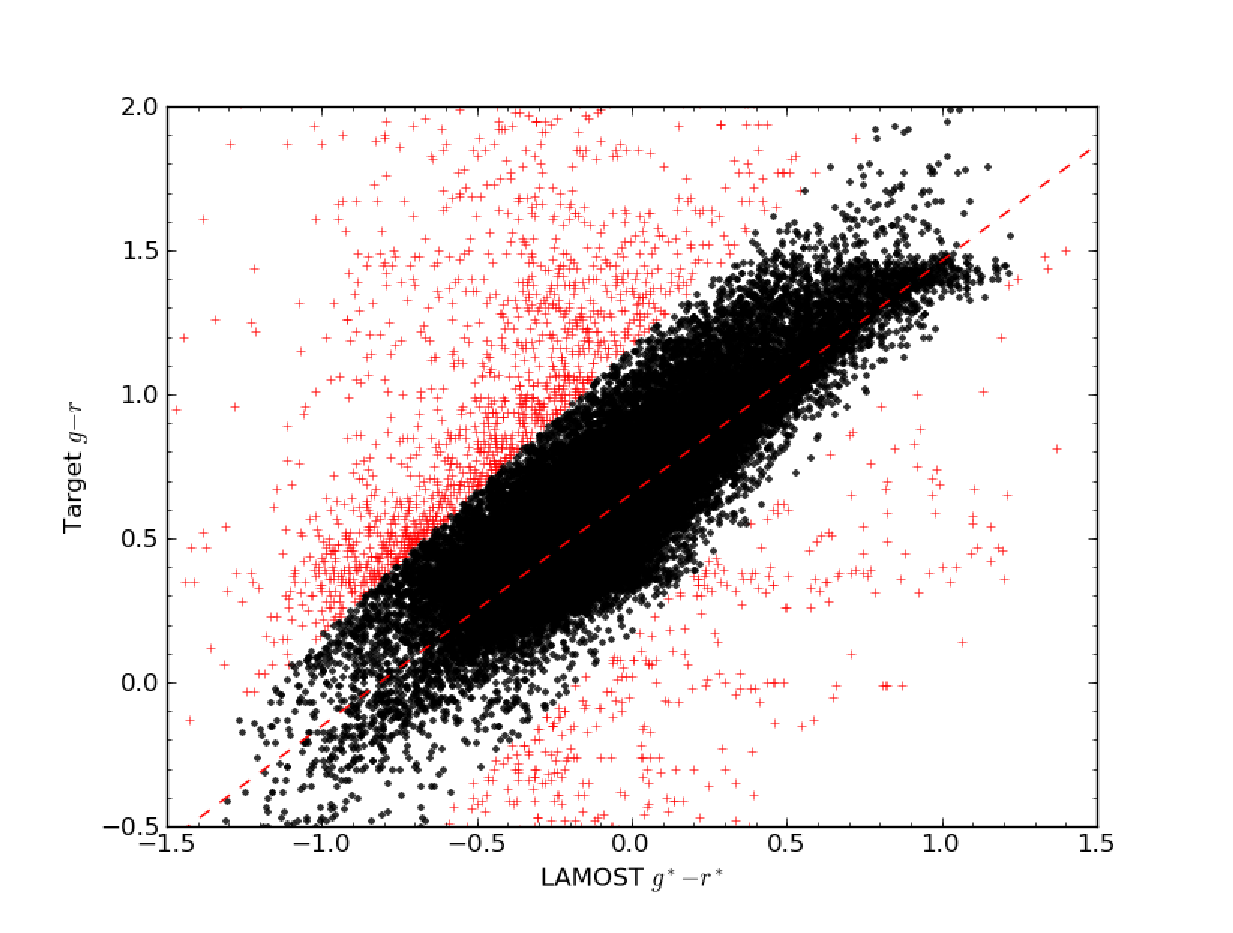
\includegraphics[width=10cm, angle=0, clip=true]{f1.eps}
   \caption{The relationship between g-r color and $g^*$-$r^*$.
   The X values are the $g^*$-$r^*$ colors and the Y values are the g-r colors  in the target catalogue.
   The red line is  derived best-fit expression as formula \ref{grrel},
   and the red points are excluded outliers while deriving the expression.
   }
   \label{Fig2}
   \end{figure}

\citet{ivezic2008milky} derived a relation between the Teff and the color g-r in the range of $-0.3 < g-r < 1.3$ For SDSS spectra:
\begin{equation}
 Log_{10} (T_{eff}/K)=0.0283* (g-r)^3 + 0.0488* (g-r)^2 - 0.316* (g-r) +3.882
 \label{grrel}
\end{equation}
Thus, we are able to derive a expression shown in formula \ref{eq3} between effective temperature $T_{eff}$ and the color g$^*$-r$^*$ using the  formula \ref{grrel}  and the  formula \ref{eq2} as:
\begin{equation}
 Log_{10} (T_{eff}/K)=0.0283* (g^*-r^*)^3 + 0.0318* (g^*-r^*)^2 - 0.203* (g^*-r^*) +3.696
 \label{eq3}
\end{equation}

For 5,220,138 A,F, G and K-type spectra, their effective temperatures , surface gravities  and metallicities determined by the LAMOST Stellar Parameter pipeline (LASP, see  \citet{wu2011automatic}) are provided.
The relationship between $g^*$-$r^*$  color and $T_{eff}$ is shown in  Figure \ref{Fig3}
and the derived   polynomial expression is as shown in formula \ref{eq4}:
\begin{equation}
Log_{10} (T_{eff}/K)=0.0432* (g^*-r^*)^3 +0.0107* (g^*-r^*)^2 -0.165* (g^*-r^*) +3.746
\label{eq4}
\end{equation}

As shown in Fig.\ref{Fig3}, the formulas \ref{eq3} and \ref{eq4}  nearly  coincide with each other in the range of Teff [5500K,7000K].
Thus, the defined $g^*$-$r^*$ color is also be a good indicator of Teff,
which is used as a criterion of dividing groups of the slected spectra.
 \begin{figure}
   \centering
   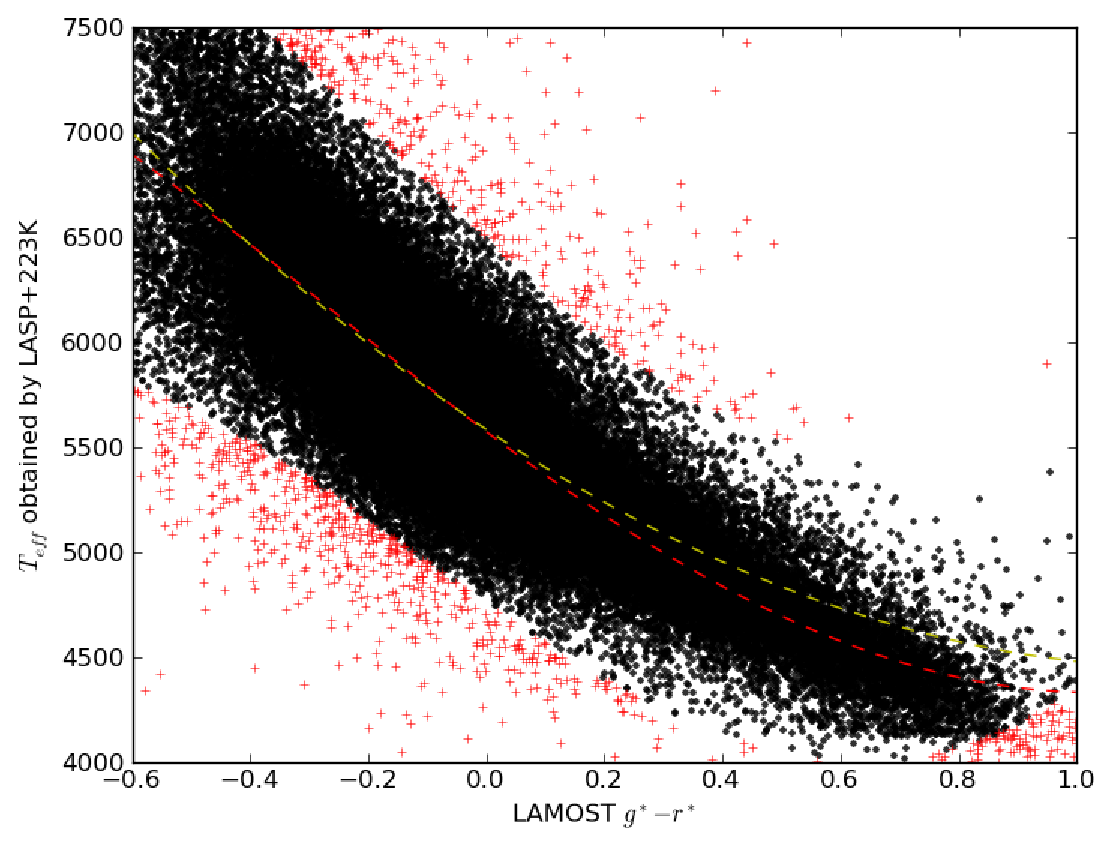
\includegraphics[width=10cm, angle=0,clip]{f3.eps}
   \caption{The relationship between the $g^*$-$r^*$  color and the $T_{eff}$.
   The $T_{eff}$ is added by 223K to decrease the system inconsistency between SSPP and LASP \citep{wu2011automatic}.
    The yellow line is the expression as formula \ref{eq3}.
     The red line is  derived best-fit expression as formula \ref{eq4},
     and the points in red are excluded outliers while deriving the expression.   }
   \label{Fig3}
   \end{figure}


\subsubsection{Group dividing criteria}

To construct different kinds of templates, we gather these spectra in 233 different groups by the proposed $g^*$-$r^*$ color and the stellar subclass classified by the pipeline using the current template library.

As discussed above, the proposed $g^*$-$r^*$ color is a good indicator of Teff.
Therefore, we select these spectra with $g^*$-$r^*$ in  the range[-1.5,2.0] and divide all spectra into 175 groups with 0.02 mag width interval.
These groups are marked with group-id from 1 to 175.
The number distribution is shown in Figure \ref{Fig4}.
 \begin{figure}
   \centering
   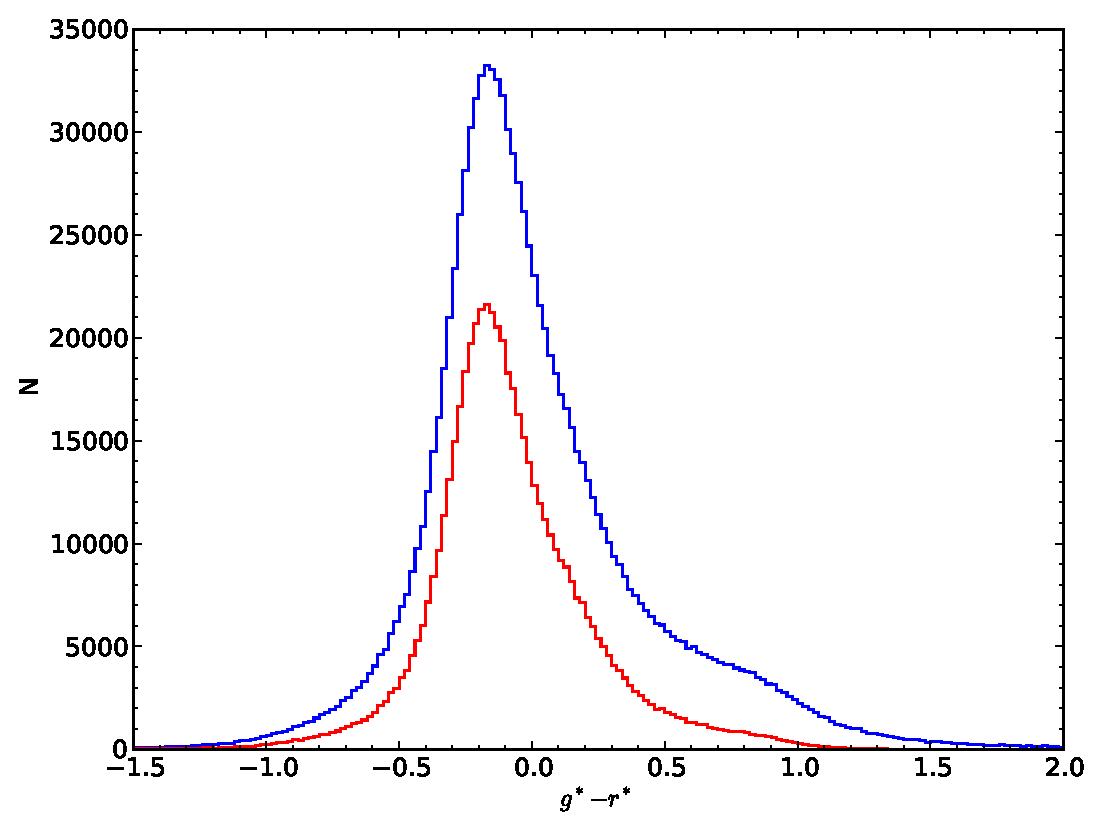
\includegraphics[width=10cm, angle=0,clip]{f2.eps}
   \caption{The number distribution of spectra in each $g^*$-$r^*$ bin.
   The blue line is the distribution of all spectra while the red line is the distribution of the spectra with $SNR>10$.
   }
   \label{Fig4}
   \end{figure}
%\subsubsection{subclass dividing}

In addition, other 60 groups are formed by the subclass labeled by current pipeline.
After the automated processing of LAMOST spectra analysis pipeline and visual inspection,
there are 60 different stellar subclasses in our selected spectra.
%Some A-type spectra in MILES library \citep{falcon2011updated} are picked out to add into the templates.
%Consequently, there are more A-type subclasses.
These groups are marked with group-id from 176 to 233.
  \citet{yi2013m} presented a spectroscopic catalog of 67,082 M dwarfs from LAMOST Pilot Survey,
and we mark these spectra with group id from 220 to 229.
%We have divided these spectra into groups with group id as shown in Table \ref{tab1}.
  \citet{zhao201370}  presented a spectroscopically identified catalog of 70 DA white dwarfs  (WDs).
Meanwhile,  \citet{zhang2013white}  identified 230 other DA  white dwarfs,
and we combine these two catalogs and put them into group 233.
  \citet{jiang2013data} reported the identification of 10 cataclysmic variables,
and we allocate a group id 204 for these spectra.
The distribution of these groups is as shown in Table \ref{tab1}.
%
%In addition, we have changed some spectra's subclasses and add some new spectra.
%  \begin{itemize}



%\end{itemize}


\begin{table}
\bc
\begin{minipage}[]{100mm}
\caption[]{The number distribution of different subclasses\label{tab1}}\end{minipage}
\setlength{\tabcolsep}{1pt}
\small
 \begin{tabular}{clr|lclr|lclr}
  \hline\hline
Group ID&Subclass&Amount&&Group ID&Subclass&Amount&&Group ID&Subclass&Amount\\
  \hline

176&A0&94&&196&A9&4&&216&K3&77164\\
177&A0I&27&&197&A9V&2170&&217&K5&73045\\
178&A0III&407&&198&B&15&&218&K7&45839\\
179&A1IV&653&&199&B0&1&&219&K9&4\\
180&A1V&527&&200&B9&443&&220&M0&19152\\
181&A2I&10&&201&Binary&170&&221&M1&19953\\
182&A2IV&1692&&202&Carbon&178&&222&M2&17243\\
183&A2V&5761&&203&CarbonWD&6&&223&M3&9749\\
184&A3I&37&&204&CV&17&&224&M4&3860\\
185&A3IV&2084&&205&EM&63&&225&M5&855\\
186&A3V&2080&&206&F0&27808&&226&M6&412\\
187&A4III&926&&207&F2&44192&&227&M7&259\\
188&A4V&773&&208&F5&119328&&228&M8&47\\
189&A5&26&&209&F9&292830&&229&M9&66\\
190&A5I&213&&210&G0&47697&&230&O&79\\
191&A5V&1253&&211&G2&92229&&231&OB&16\\
192&A6IV&1240&&212&G5&81202&&232&WD&535\\
193&A6V&322&&213&G7&3650&&233&WD Magnetic&14\\
194&A7III&4033&&214&K0&1998&&&&\\
195&A7V&647&&215&K1&85218&&&&\\


 \hline\hline
\end{tabular}
\ec
%% place \tablecomments and \tablerefs below \end{center| and \end{center}:
%% you may leave the table-width parameter to editors or set to your actual size
%\tablecomments{0.86\textwidth}{'-' in subclass and amount means the corresponding group is neglected.}
\end{table}



%Consequently, there are 233 groups in total.
%The group with less number are not neglected to avoid excluding some relatively rare types of stars.
\subsection{The construction of spectral templates library}
\subsubsection{Excluding outliers using LOcal Outlier Probabilities (LoOP)}
% \citet{kriegel2009loop} proposed a local outlier factor (LOF, see  \citet{breunig2000lof}) based outlier detection  method.
To construct template spectra,
233 different groups are formed by gathering similiar spectra following two criteria.
Although the spectra  in the same group are very similiar with each other, there are still some outliers existing in each group for many reasons,
including the effect of instellar extinction on the continiuum, strong noises, existence of unusual spectral features and other issues.
Obviously, these outliers should be excluded to generate much purer spectra for construction of template spectra.

In our work, the LOcal Outlier Probabilities (LoOP, see \cite{kriegel2009loop} ) method is used to exclude these outliers.
LoOP is a local density based method that uses statistical concepts to output the final score.
The LoOP score represents the probability that a particular point is a local density outlier.
The the detailed description of LoOP is shonw in \citep{kriegel2009loop}:
%\begin{enumerate}
%					\item    ($k$-$distance$ of an object $p$) For any
%					positive integer $k$,  the $k$-distance  (The distance measurement function used in our work is the cosine distance $d=1-\frac{A*B}{|A|*|B|}$) of object $p$, denoted as
%					$k$-$distance  (p)$, is defined as the distance $d  (p, o)$ between $p$ and
%					an object $o\in D$ such that:
%					  (i) For at least $k$ objects $o'\in{D}\setminus{p}$, it holds that $d  (p, o')\le d  (p, o)$.
%					  (ii )For at most $k$-1 objects $o'\in D\setminus p$, 	it holds that $d  (p, o')$$<$$d  (p, o)$.
%					
%					\item  ($k$-$distance$ neighborhood of an object $p$)
%					Given the $k$-$distance$ of $p$, the $k$-$distance$ neighborhood of $p$
%					contains every object whose distance from $p$ is not greater than
%					the $k$-$distance$, i.e. $N_{k}$$_-$$_{distance  (p)}  (p)=\{q\in D\setminus p\mid
%					d  (p, q)\leq k$-$distance  (p)\}$. These objects $q$ are called the
%					$k$-$nearest$ neighbors of $p$. Simplify the notation to use
%					$N_{k}  (p)$ as a shorthand for $N_k$$_{-}$$_{distance}  (p)$.
%					
%					  \item  The standard distance. $\sigma (p,N_k (p))$ is defined as the standard deviation of the distance around $p$:
%					  \begin{equation}
%					   \sigma (p,N_k (p))=\sqrt{\frac{\sum_{s\in N_k (p)}^{} d (p,s)^2}{|S|}}
%					  \end{equation}
%					
%					 \item  The probabilistic set distance. $pdist (\lambda,p,N_k{p})$ is defined as follows:
%					  \begin{equation}
%					  pdist (\lambda,p,N_k{p})=\lambda*\sigma (p,N_k (p))
%					  \end{equation}
%					
%					   \item The Probabilistic Local Outlier Factor PLOF.  $PLOF_{\lambda,S (p)} (p)$ represents the ratio of the density estimation:
%					  \begin{equation}
%					   PLOF_{\lambda,S (p)} (p)=\frac{pdist (\lambda,p,N_k (p))*|N_k (p)|}{\sum_{s\in N_k (p)}^{}pdist (\lambda,s,N_k (s))}-1
%					  \end{equation}
%					
%					  \item The aggregate Probabilistic Local Outlier Factor nPLOF.  This is the scaling factor that makes the score independent from any distribution:
%					  \begin{equation}
%					   nPLOF=\lambda*\sqrt{\frac{\sum_{p\in D}^{}PLOF_{\lambda,S (p)} (p)^2}{|D|}}
%					  \end{equation}
%					
%					  \item The Local Outlier Probability:
%					  \begin{equation}
%					   LoOP_{N_k{p}} (p)=max (0,erf\frac{PLOF_{\lambda,S} (p)}{nPLOF*\sqrt{2}})
%					  \end{equation}
%\end{enumerate}


%In our work, we use LoOP to exclude outliers in each group to get a better template spectra.

\subsubsection{The spectra reconstruction using Principal Component Analysis (PCA)}
The Principal Component Analysis  (PCA, see \cite{jolliffe2002principal}) is a mathematical procedure that uses an orthogonal transformation to convert a set of observations of possibly correlated variables into a set of values of linearly uncorrelated variables called principal components.
The number of principal components is less than or equal to the number of original variables.
This transformation is defined in such a way that the first principal component has the largest possible variance  (that is,  accounts for as much of the variability in the data as possible).

As a viable tool, Principal Component Analysis (PCA) has been applied  in the classification of spectra \citep{whitney1983principal,bailer1998automated,yip2004spectral,almeida2013automated} by  reducing the dimensionality of the original spectral data to very few components.
PCA are also able to successfully reconstruct the original spectra by using the first few components \citep{singh1998stellar}.
In our work, PCA is used to reconstruct the original spectra to improve the similarity of spectra in the same group.
%and each succeeding component in turn has the highest variance possible under the constraint that it be orthogonal to   (i.e.,  uncorrelated with) the preceding components.	
				      %The detailed description of the PCA method is discussed in \cite{whitney1983principal,jolliffe2002principal}.
				
				     % As a viable tool, Principal Component Analysis (PCA) has been applied  in the classification of spectra \citep{whitney1983principal,bailer1998automated,yip2004spectral,almeida2013automated}.
%In addition,  \cite{tu2009new,tu2010method,jiang2013data,wei2013mining} have used PCA to do the data dimension reduction in finding relatively rare objects.
% \cite{mcgurk2010principal} applied PCA to 200,000 stellar spectra obtained by the Sloan Digital Sky Survey  (SDSS).
%They discussed correlations of eigen-coefficients with metallicity and gravity estimated by the Sloan Extension for Galactic Understanding and Exploration Stellar Parameters Pipeline (SSPP) \citep{lee2008segue}.

\subsubsection{The steps to construct the template library}
We use the following ten steps to construct the new stellar template library for spectra analysis pipeline
(note that the number in an bracket is the number of remaining spectra after this step):
\begin{enumerate}
\item For the groups with more than 5,000 spectra, only first 5,000 spectra with the largest SNR are selected.[525,723]
\item Remove the readshift of each spectrum, unify wavelength to 3800\AA-9000\AA \ with fixed step 1\AA\ (the amount of all sampling points is N=5201) and  get the unified flux $F$.
  \item Exclude these spectra existing $F\le0$  and normalize the remaining spectra $F$ as follows [489,137]:
       \begin{equation}
        F_i=\frac{F_i}{\sqrt{\sum\limits_{j=1}^{N}F_i^2}}
       \end{equation}
 \item Calculate LoOP for each group
 \item These spectra with  $LoOP\ge0.4$ are excluded. [415,381]
		

      \item Apply the PCA to the remaining spectra in each group to  obtain a feature matrix $T$ and the corresponding eigen values $\lambda$.
      \item Select the first $k$-th principal components (eigen spectra) while the variance contribution rate $\mu$ :
      \begin{equation}
       \mu=\frac{\sum\limits_{i=1}^{k}\lambda_i}{\sum\limits_{i=1}^{N}\lambda_i}>\theta
      \end{equation}
      where $\theta$ is a fixed given threshold  (0.99 is used in our work).
       $k$ is set to 2 when $k=1$.

     \item Reconstruct each remaining spectra using obtained first $k$ principal components
     \item Calculate LoOP of remaining reconstructed spectra in each group again and exclude these spectra with $LoOP\ge0.2$. [367,248]

      \item Take the SNR weighted average spectrum as the template spectrum in each group.
     \end{enumerate}

\subsubsection{Class Labeling}
Following  above ten steps, the template spectra are successfully constructed in 216 groups  (nearly 92\%).
Other 17 groups fail mainly because of lacking enough high quality spectra.
Each spectrum should be labeled a subclass for latter usage in classification.
We compare these spectra with three libraries and then label each spectrum a subclass.

 \citet{danks1994atlas} presented spectra  for MK standards in the wavelength range    5800\AA-10200\AA.
The stars cover the normal spectral types from O to M and    luminosity types I, III, and V.
The projected slit width along the dispersion is about 4\AA\ and the resolution R is about 1200.
Two wavelength ranges [7500\AA,7700\AA] and [6800\AA,7000\AA] are masked to get rid of the strong telluric lines left in the spectra.
We decrease the resolution of our templates to R~1200 by convolving a gaussian function.
All template spectra and standard spectra are unified into the wavelength range [6100\AA,9000\AA] with a fixed step 4\AA.
%For each template spectrum, the first four  closest  are chosen and the corresponding spectra are drawn together with the template spectra.
%Those figures are used for following visual inspection.

 \citet{bolton2012spectral} described the detail of the pipeline for SDSS III and published the template used on the web page\footnote{\url{http://www.sdss3.org/svn/repo/idlspec2d/tags/v5_4_45/templates/}}.
For stellar spectral classification,  123 templates created from the full database of Indo-U.S. spectra are provided.
Each spectrum are labeled a MK class by matching with POLLUX database.
The resolution R of these 123 spectra is about 2000 and the wavelength coverage is from 3500\AA\ to 11200\AA.
These spectra are unified into the wavelength range [3800\AA,9000\AA] with a fixed step 1\AA\ similar with the spectra in the library .
%Similarly, for each template spectrum, the first four  closest are chosen and the corresponding spectra are drawn together with the template spectra.
%And those figures are also used for following visual inspection.

As introduced above, the current library used for stellar classification in LAMOST contains 36 classes plus 20 subclasses specially for A-type star.
The resolution R of these 56 spectra is about 2000 and the wavelength coverage is from 3800\AA\ to 9200\AA.
These spectra are unified into the wavelength range [3800\AA,9000\AA] with a fixed step 1\AA\ similar with the spectra in the library .
%Similarly, for each template spectrum, the first four  closest are chosen and the corresponding spectra are drawn together with the template spectra.
%And those figures are also used for following visual inspection.

Each template spectrum is visually inspected by checking the three figures drawn above.
And then each spectrum is labeled a MK class.
Meanwhile, those template spectra with bad data or low SNR are excluded.
Finally,  there are 164 spectra and 65 different MK classes are left in the template library.


\section{Results and  discussions}
\label{sect:Results}
A updated library is formed after adding some spectra of new subclasses and replacing some spectra.
These spectra of the types not existing in our library are left.
The library of the current version (V1.0) is publicly available on the web site\footnote{\url{http://sciwiki.lamost.org/lamost_sctl/v1}}.
The current library has been used in the new new version of LAMOST 1D pipeline for spectra after data release one.
\subsection{Examples}
\label{sect:Examples}
Here we choose four typical groups  (Group 59,180 ,207 and 237)  to  discuss in detail.
The main information of these groups is shown in Table.\ref{tab2}.
The MK classes are F6V, A1IV, CV and M2 respectively.
The finally constructed template spectra of these groups are  shown in Fig.\ref{Fig6}.


\begin{table}
\bc
\begin{minipage}[]{100mm}
\caption[]{The main information of groups 59,180, 207 and 237\label{tab2}}\end{minipage}
\setlength{\tabcolsep}{1pt}
\small
 \begin{tabular}{c|r|r|c|c|c|c}
  \hline\hline
Group ID&All spectra&used spectra&Subclass&Subclass1&Subclass2&Subclass3\\
  \hline
59  &18534    &3048  &F4V    &F3V/F5V  &F8III-IV &F5   \\
180 &653    &381  &A1IV    &A4V/A1V  &A2V&A1V    \\
207 &27     &13  &CV    &-  &-&-    \\
237 &17231     &325  &M2    &M1/M0  &M1.5V/M3V&M2/M1    \\
 \hline\hline
\end{tabular}
\ec
%% place \tablecomments and \tablerefs below \end{center| and \end{center}:
%% you may leave the table-width parameter to editors or set to your Vactual size
\tablecomments{0.86\textwidth}{Subclass is the finally labeled MK class.
Subclass1 is the best fit Mk class with  \citet{bolton2012spectral}.
Subclass2 is the best fit Mk class with  \citet{danks1994atlas}.
Subclass3 is the best fit Mk class with  \citet{luo2012dr1}.}
\end{table}
 \begin{figure}
   \centering
   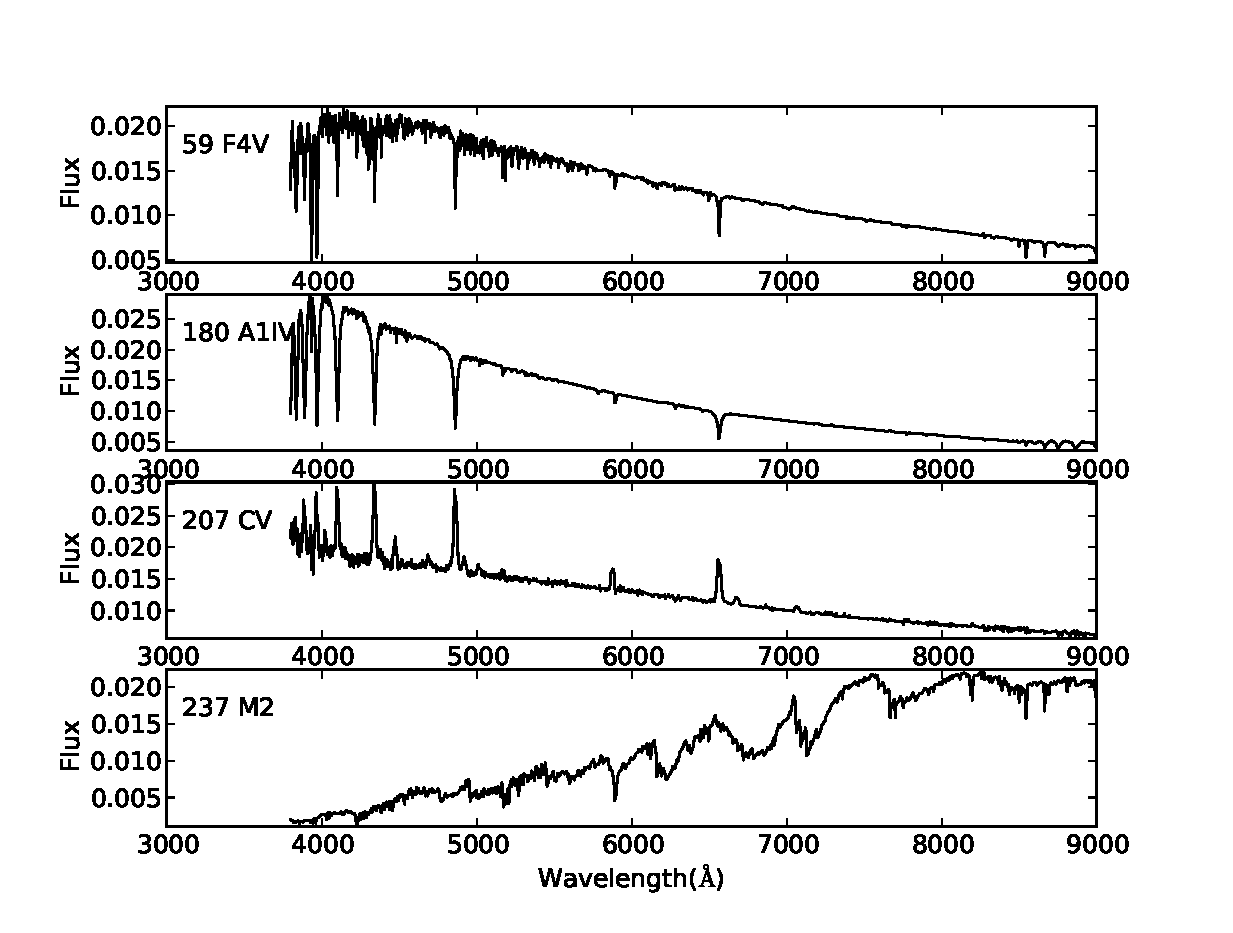
\includegraphics[width=10cm, angle=0,clip]{f6.eps}
   \caption{The template spectra of groups 59,180, 207 and 237.
   }
   \label{Fig6}
\end{figure}

\textbf{Group:59}
This group contains the spectra in the color $g^*$-$r^*$ range [-0.34,-0.32].
There are totally 18,534 spectra and 3,048 spectra are selected from the first 5,000 spectra with the highest SNR.
As shown in Fig \ref{Fig91}, the spectrum is very close to F3V/F5V in  \citet{bolton2012spectral}.
Consequently, the template spectrum is labeled as 'F4V'.
\begin{figure}
   \centering
   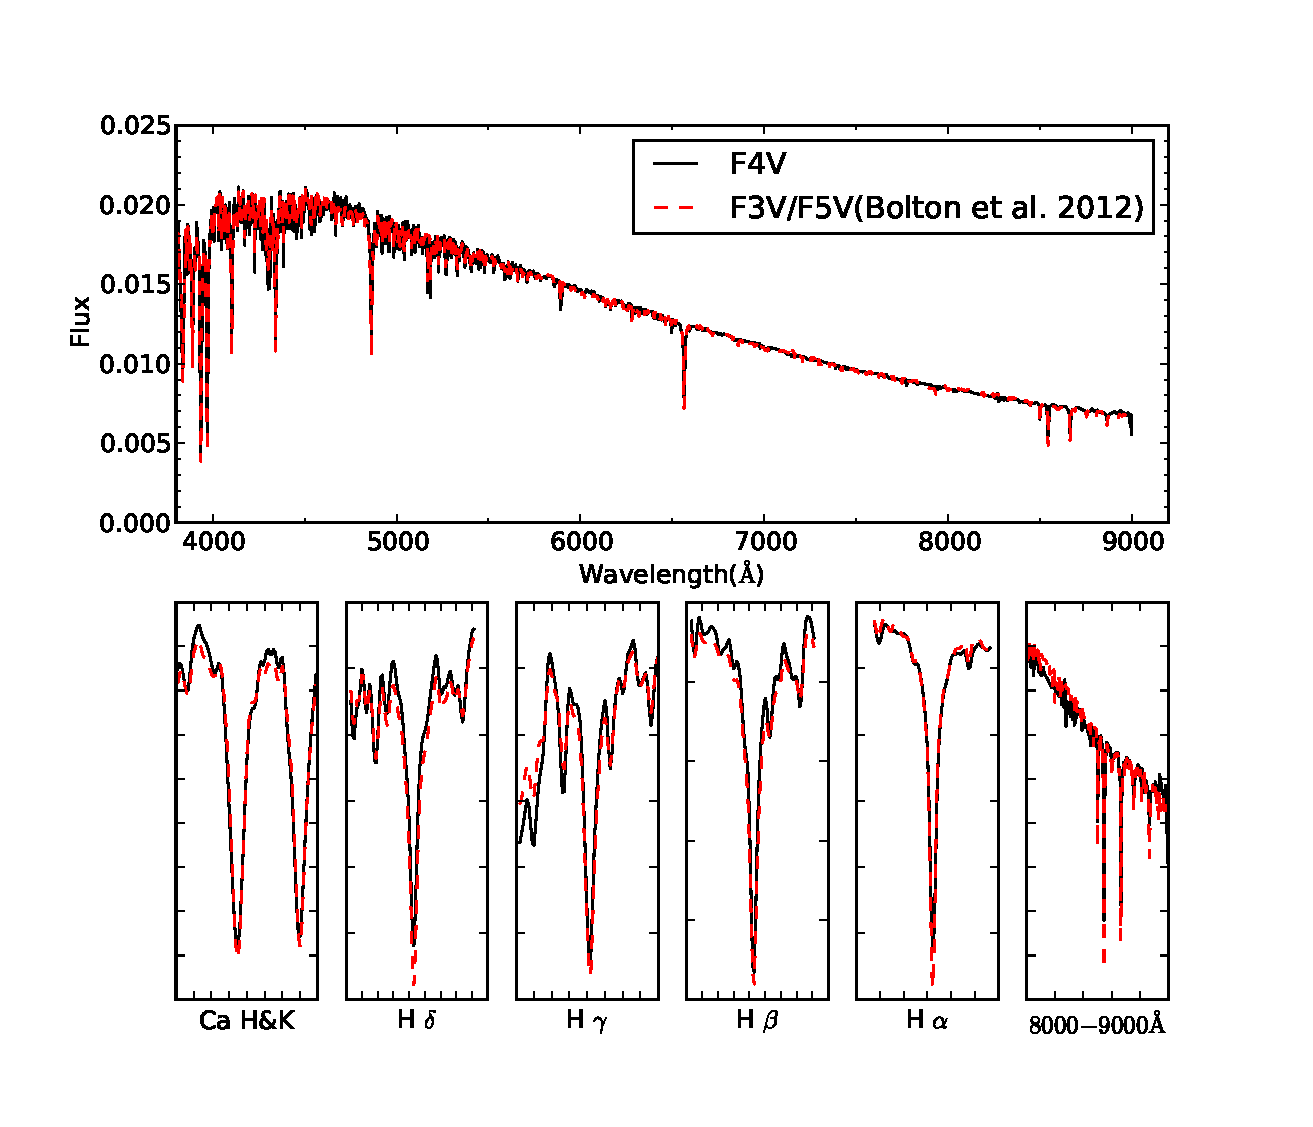
\includegraphics[width=10cm, angle=0,clip]{f91.eps}
   \caption{The comparison of the template spectrum in group 59 with  F3V/F5V in  \citet{bolton2012spectral}.
The black line is the spectrum constructed in our work.
The red one is the closest spectrum in  \citet{bolton2012spectral}.
   }
   \label{Fig91}
\end{figure}

As shown in Fig \ref{Fig71},  the variance of the first  principal component  exceeds more than 99\% of the total variance of the original data.
That is due to the high similarity of the spectra in the group.
Consequently, the reconstructed spectra using first two  principal components are nearly similar to the origin spectra (see Fig \ref{Fig81}).

 \begin{figure}
   \centering
   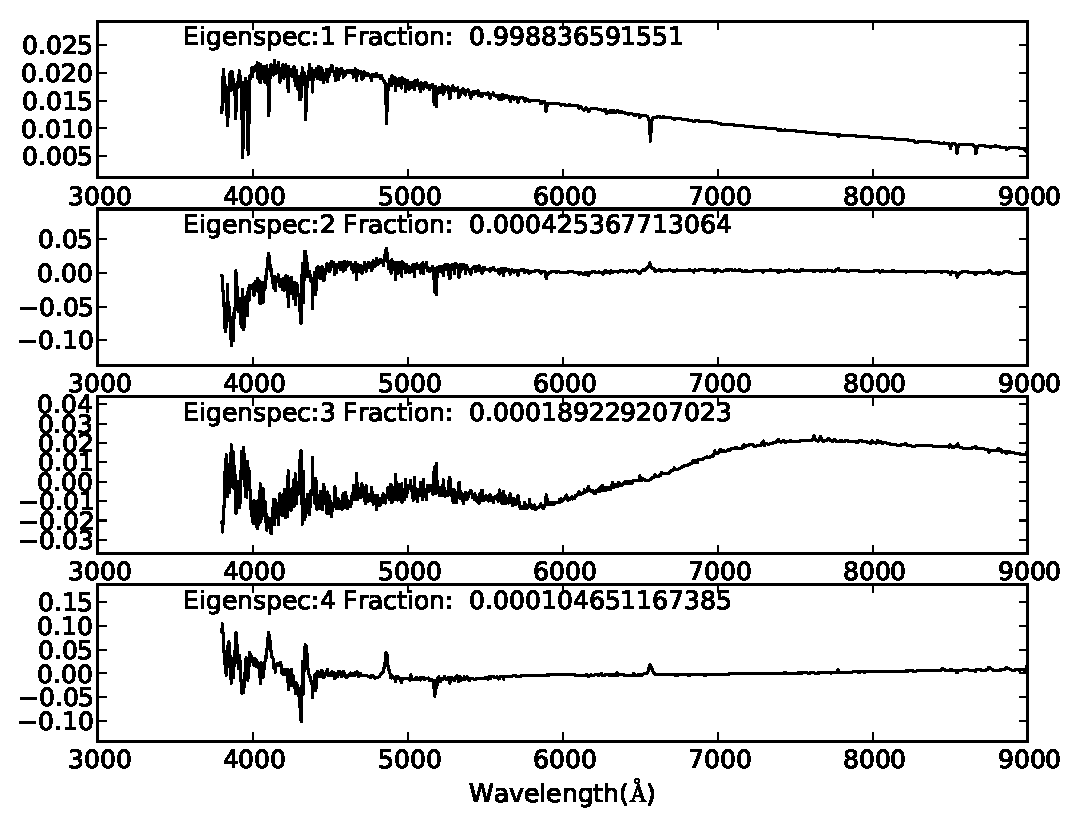
\includegraphics[width=10cm, angle=0,clip]{f71.eps}
   \caption{The first four eigen spectra (principal components) of group 59.
   }
   \label{Fig71}
\end{figure}

 \begin{figure}
   \centering
   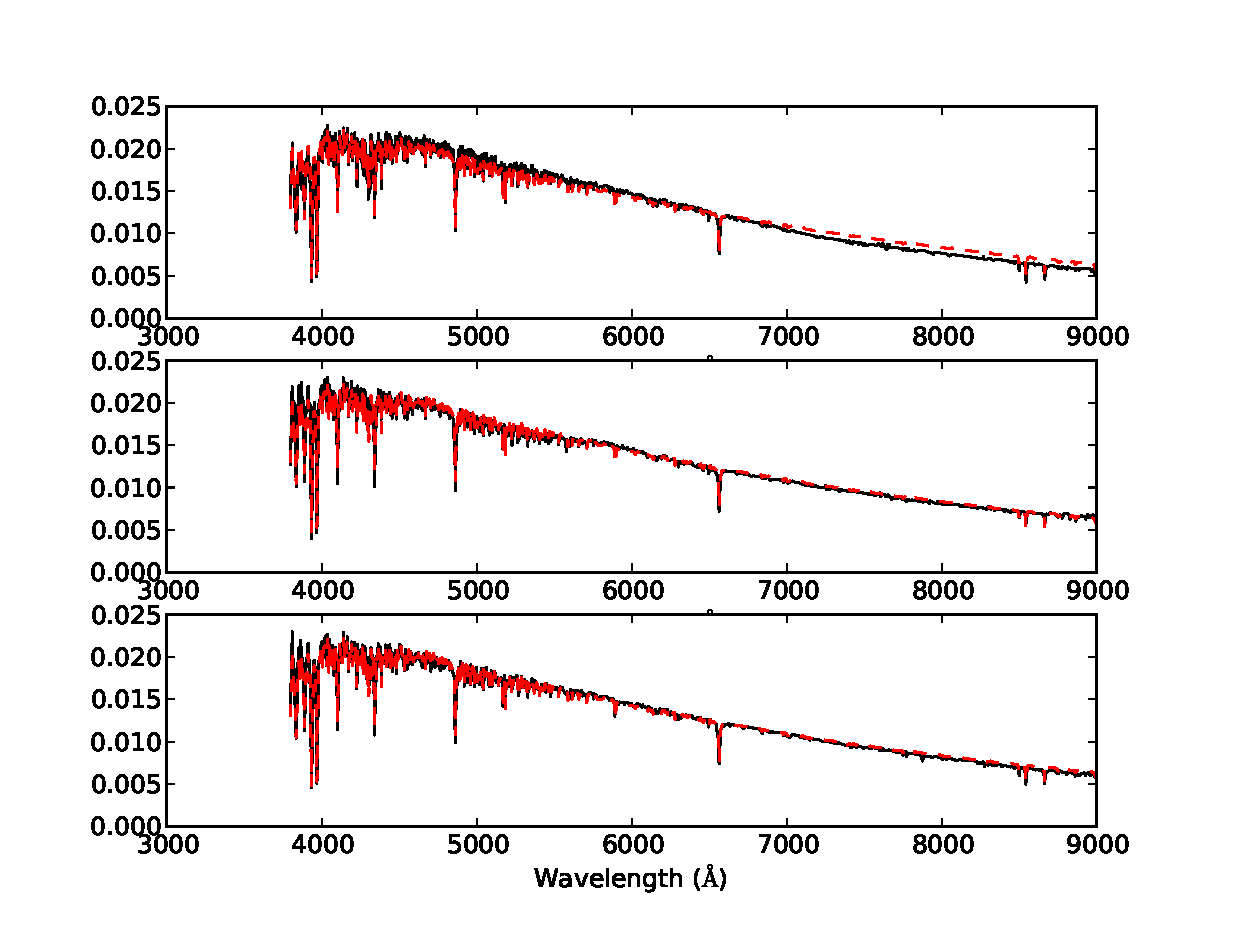
\includegraphics[width=10cm, angle=0,clip]{f81.eps}
   \caption{Three examples of reconstructed spectra in group 59
   }
   \label{Fig81}
\end{figure}


\textbf{Group:180}
This group contains the spectra classified as `A1IV' by pipeline.
There are totally 653 spectra and 381 spectra are selected.
The spectrum is labeled as `A1IV' following the group selection criteria.
As shown in Fig \ref{Fig92}, the SNR of the template is a little larger than the template in  \citet{luo2012dr1} while these two spectrum are nearly close to each other.
\begin{figure}
   \centering
   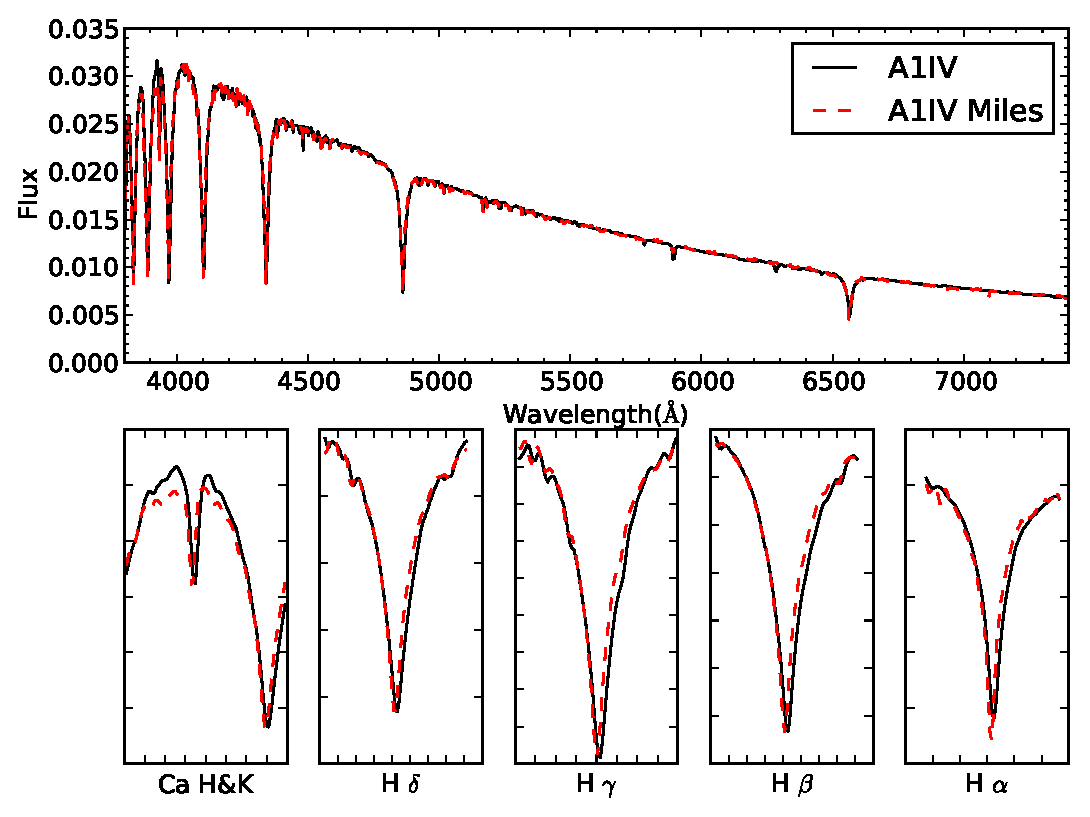
\includegraphics[width=10cm, angle=0,clip]{f92.eps}
   \caption{The comparison of the template spectrum in group 59 with  A1IV in  \citet{luo2012dr1}.
The black line is the spectrum constructed in our work.
The red one is the closest spectrum in  \citet{luo2012dr1}.
   }
   \label{Fig92}
\end{figure}

Similar with group 59, the variance of the first  principal component also exceeds more than 99\% of the total variance of the original data (see Fig \ref{Fig72}).
However, there are not as many spectra as in group 59.
Consequently, some  spectra are not well reconstructed (as shown in Fig \ref{Fig82}).
In spite of this, the template spectrum is well constructed after excluding these badly reconstructed spectra.

%The results of this group show that
 \begin{figure}
   \centering
   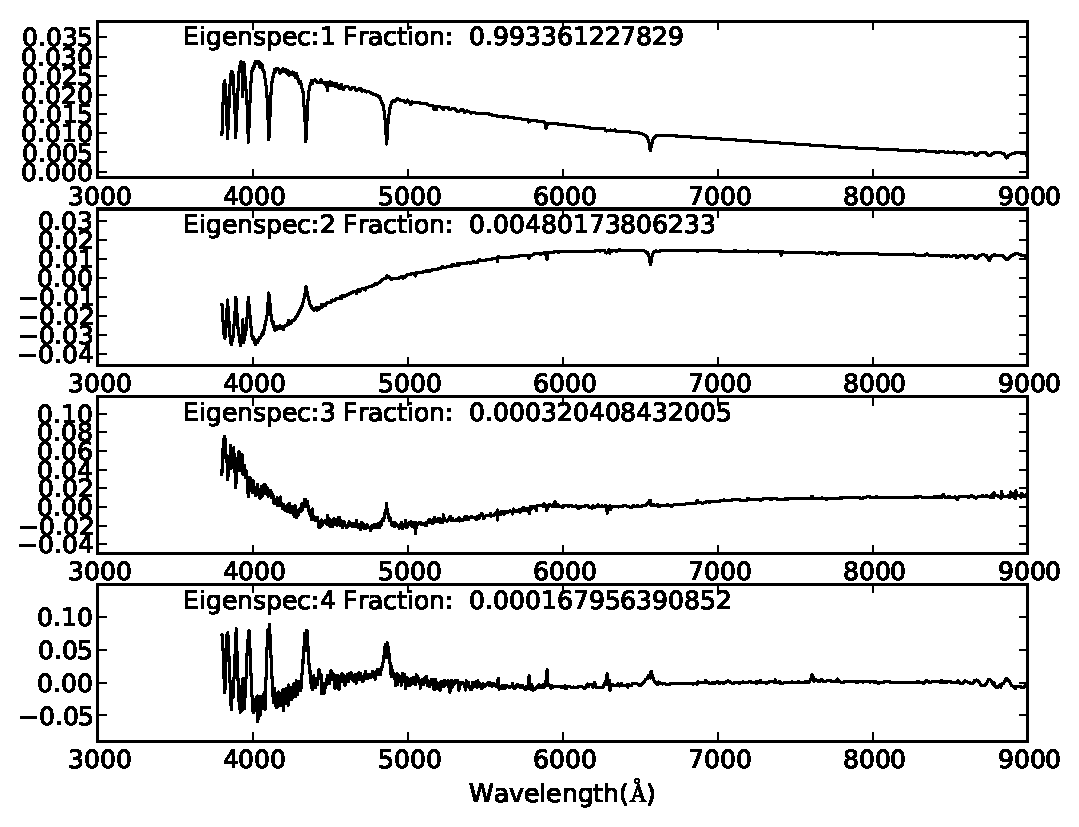
\includegraphics[width=10cm, angle=0,clip]{f72.eps}
   \caption{The first four eigen spectra (principal components) of group 180.
   }
   \label{Fig72}
\end{figure}

 \begin{figure}
   \centering
   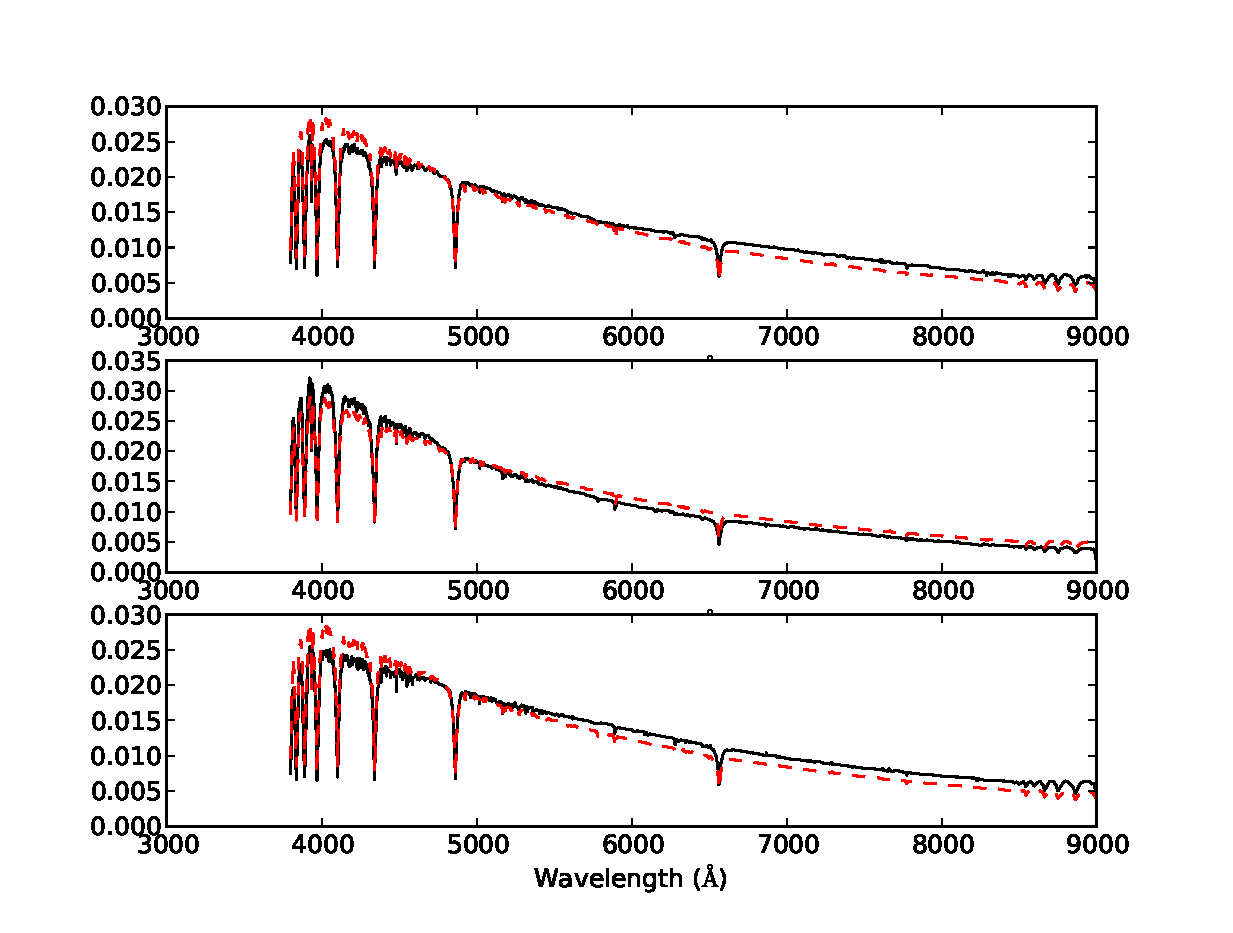
\includegraphics[width=10cm, angle=0,clip]{f82.eps}
   \caption{Three examples of reconstructed spectra in group 180
   }
   \label{Fig82}
\end{figure}


\textbf{Group:207}
This group contains the spectra classified as `CV'.
There are totally 27 spectra and 13 spectra are selected.
The spectrum is labeled as `CV' following the group selection criteria.

Compared with normal stars, the spectra of CV stars are these with strong hydrogen Balmer and helium emission lines that typically signify ongoing accretion.
As shown in Fig \ref{Fig73}, the first two principal components show obvious and strong emission lines and the sum of the variances of these two  principal components  exceeds more than 99\% of the total variance of the original data.
Compared to normal stars misclassified as 'CV', the spectra of CV stars are almost faultlessly reconstructed (see Fig \ref{Fig83}).
And then these misclassified spectra are excluded in the next following steps.
 \begin{figure}
   \centering
   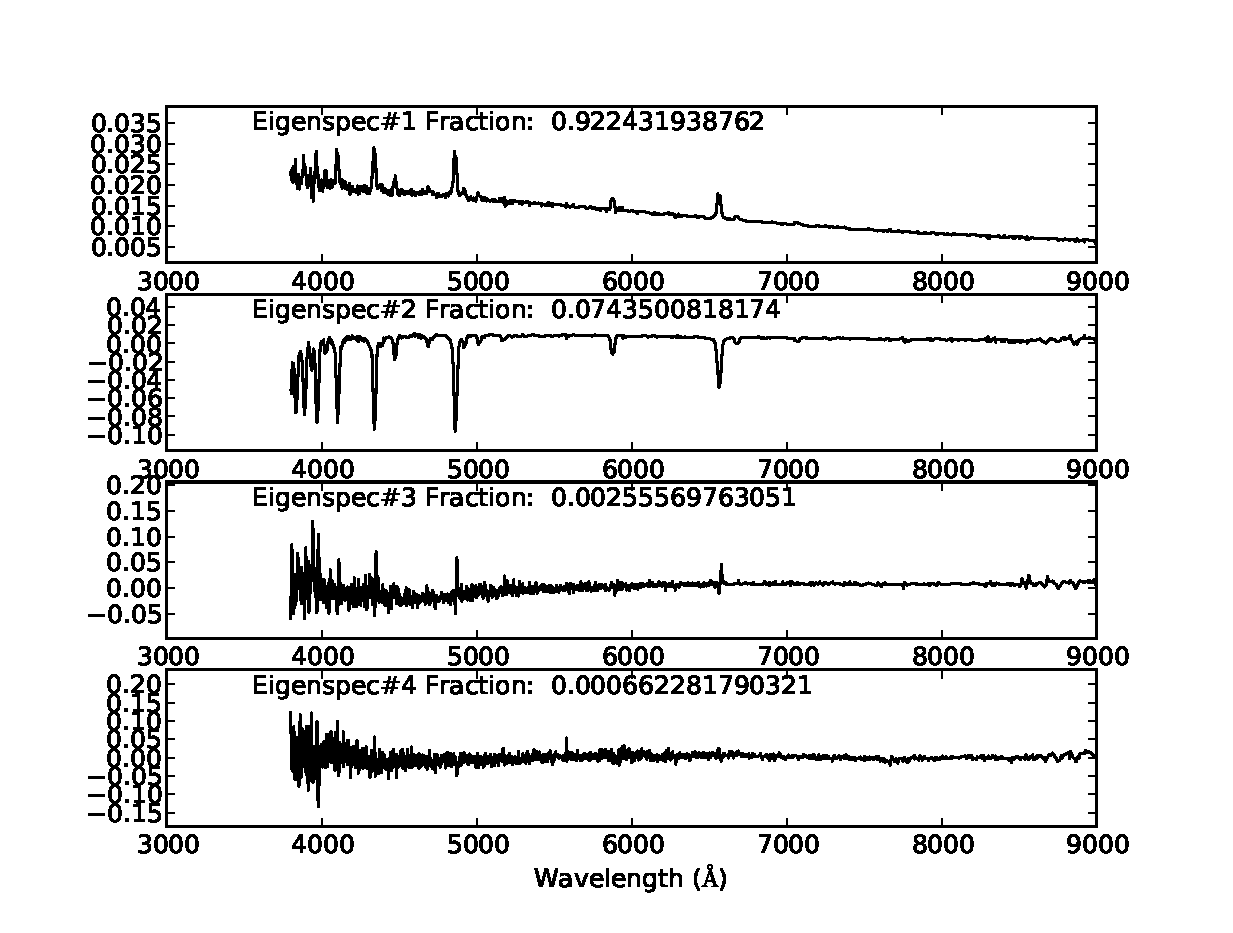
\includegraphics[width=10cm, angle=0,clip]{f73.eps}
   \caption{The first four eigen spectra (principal components) of group 207.
    Note that the strong lines in eigen spectra 2 are emission lines not absorption lines.
   }
   \label{Fig73}
\end{figure}

 \begin{figure}
   \centering
   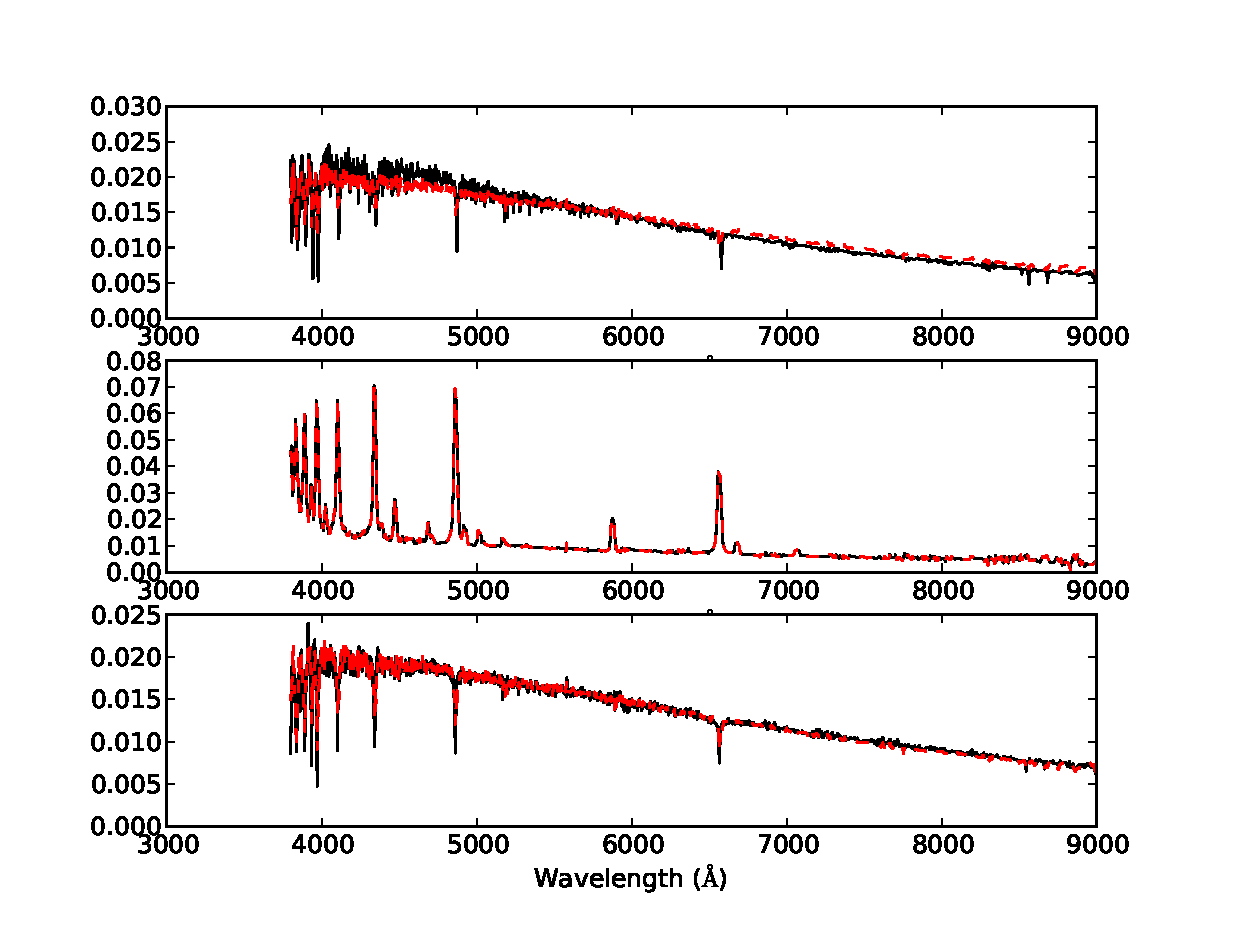
\includegraphics[width=10cm, angle=0,clip]{f83.eps}
   \caption{Three examples of reconstructed spectra in group 207.
   }
   \label{Fig83}
\end{figure}
\textbf{Group:237}

This group contains the spectra classified as `M2'.
%All M-type spectra are visually inspected to classify the subclass.
There are totally 17,231 spectra and 325 spectra are selected from the first 5,000 spectra with the highest SNR.
Due to the existence of wavelength points with $flux\le0$, a large amount of  spectra are excluded in this group.
The spectrum is labeled as `M2' following the group selection criteria.



As shown in Fig \ref{Fig74}, the sum of the variances of the first two principal components  exceeds more than 99\% of the total variance of the original data.
The selected spectra are not well reconstructed in the blue arm (as shown in Fig \ref{Fig84}).
In spite of this, the template spectrum is also well constructed.


To check the quality, we choose the M2-type template spectrum in the current template library \citep{wang2010calibration} and compare it with the template spectrum of group 237 (see Fig \ref{Fig94} upper panel).
 \citet{bochanski2007low}  presented template spectra of low-mass  (M0-L0) dwarfs derived from over 4000 Sloan Digital Sky Survey spectra.
We choose the M2-type template spectrum and alsoe compare it with the template spectrum of group 237 (see Fig \ref{Fig94} bottom panel).
As shown in Fig \ref{Fig94}, we can infer that our constructed M2-type spectrum is a little better than these two spectra.


 \begin{figure}
   \centering
   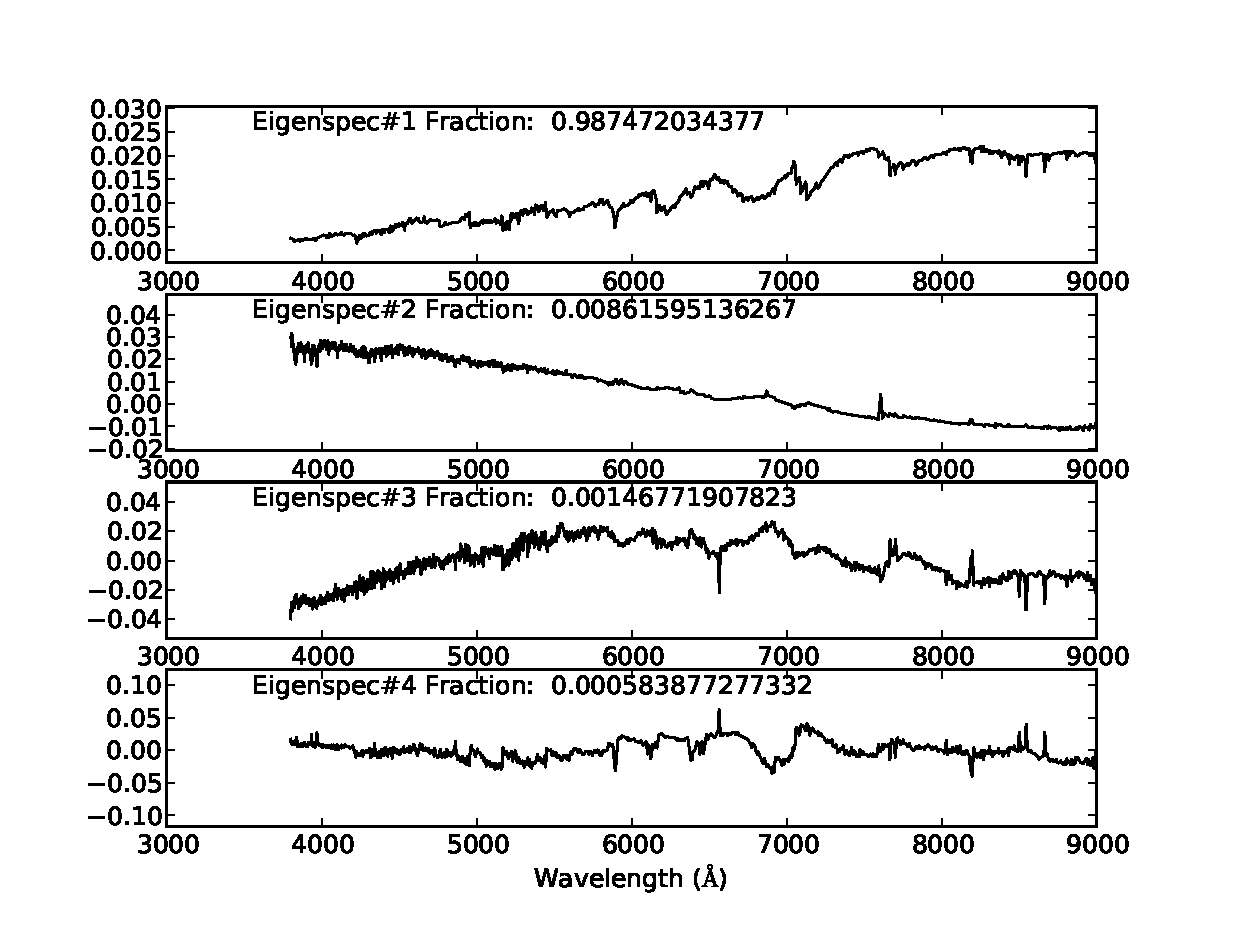
\includegraphics[width=10cm, angle=0,clip]{f74.eps}
   \caption{The first four eigen spectra (principal components) of group 237.
   }
   \label{Fig74}
\end{figure}

 \begin{figure}
   \centering
   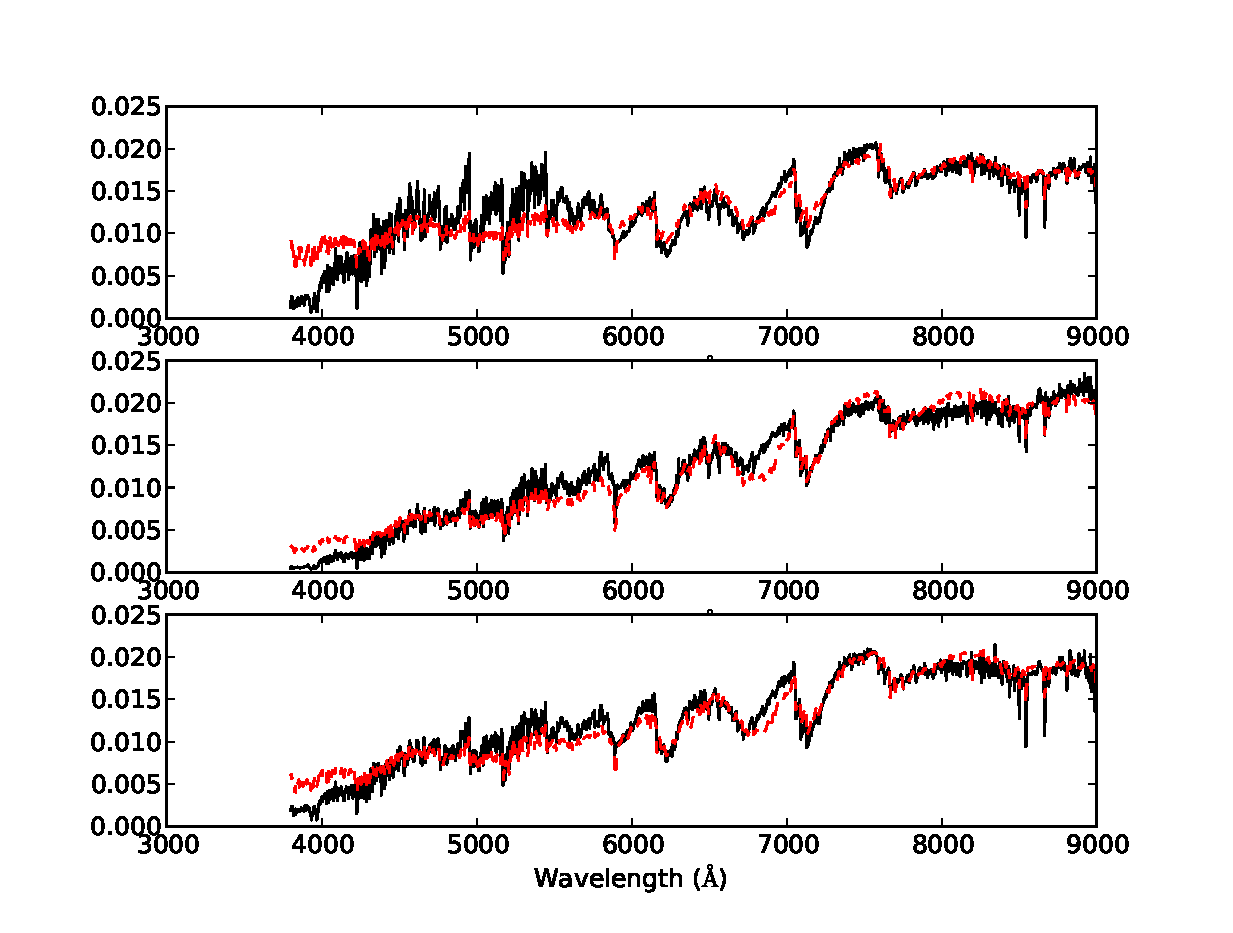
\includegraphics[width=10cm, angle=0,clip]{f84.eps}
   \caption{Three examples of reconstructed spectra in group 237.
   }
   \label{Fig84}
\end{figure}

 \begin{figure}
   \centering
   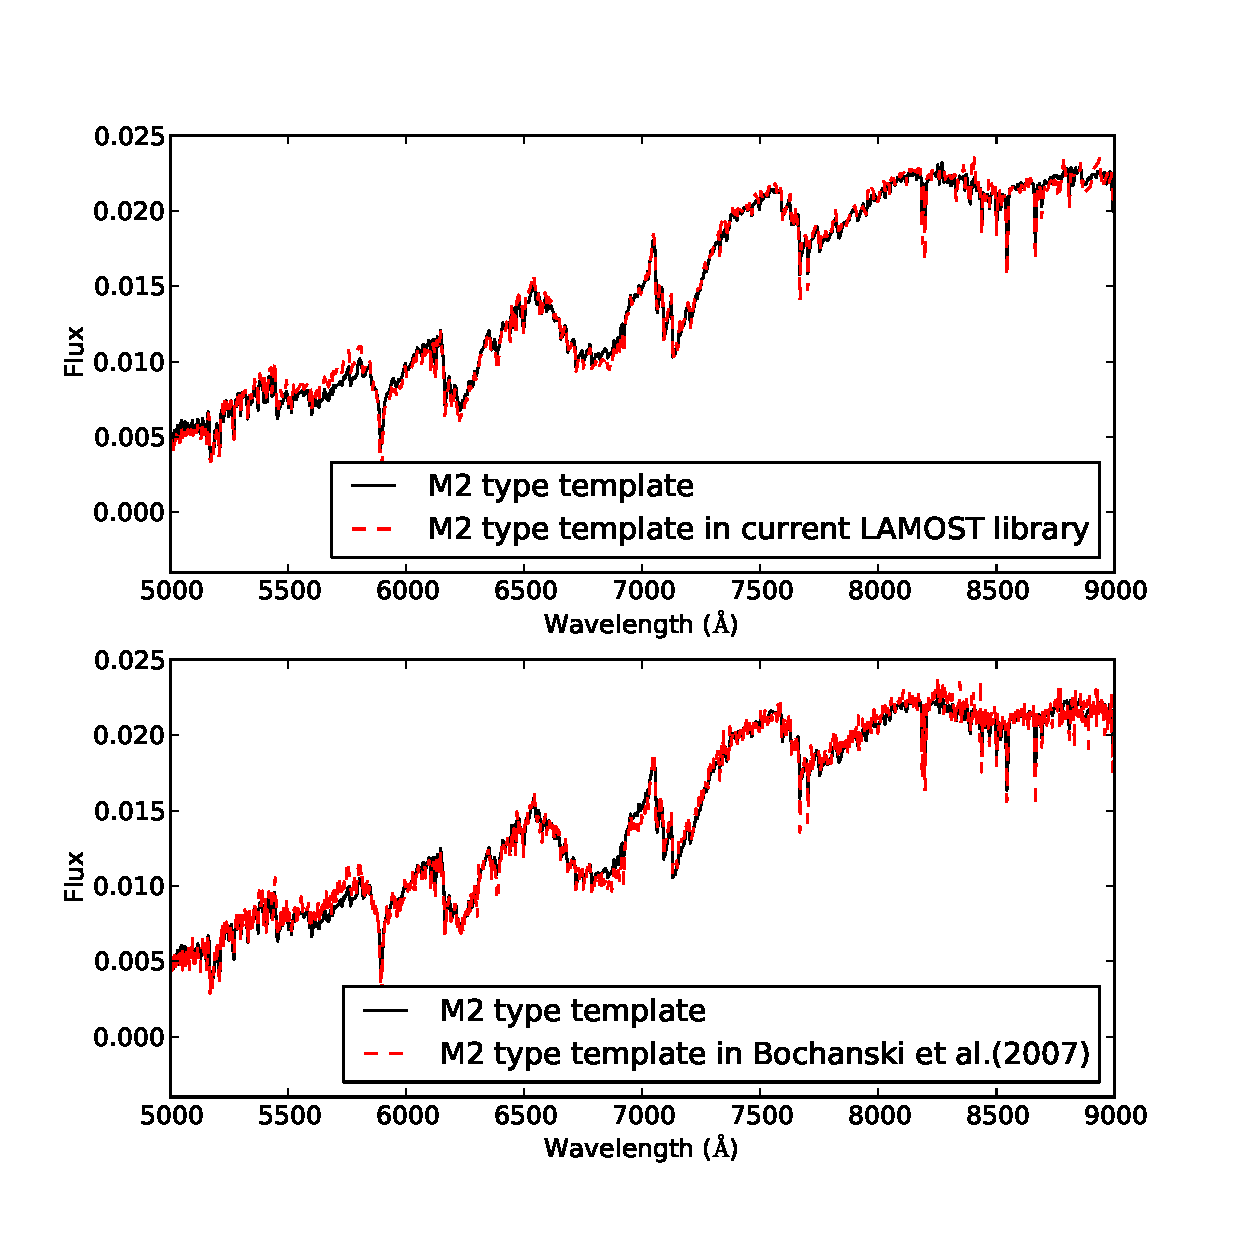
\includegraphics[width=10cm, angle=0,clip]{f94.eps}
   \caption{The comparison of the template spectrum in group 59 with  M2 in  \citet{bochanski2007low}.
The black line is the spectrum constructed in our work.
The red one is the closest spectrum in   \citet{bochanski2007low}.
   }
   \label{Fig94}
\end{figure}

%\label{sect:Comparisons}
%\subsection{Comparison with current templates}
%The current version of LAMOST 1D pipeline \citep{luo2004design,wang2010calibration} uses a template library obtained from selected SDSS spectra, which contains 36 different types of stellar spectra.
%
%
%\subsection{Comparison with  \citet{bochanski2007low}}
%
%Compare with

%There are also some other types of stellar spectra group
\subsection{Discussions}
\subsubsection{Comparison with  \cite{mcgurk2010principal}}
 \cite{mcgurk2010principal} applied PCA  to about 100,000 SEGUE spectra by dividing all spectra into 55 different bins.
For each bin, the first four eigenspectra are published and the first one is a high SNR mean spectra.
For the template spectra in all groups, to check the difference, we use similar method as MK class labeling to  find three closest mean spectra in  \cite{mcgurk2010principal}.
As our  color range is wider than  \cite{mcgurk2010principal}, not all template spectra are similar with these in  \cite{mcgurk2010principal}.
As shown in Table \ref{tab3}, the groups with groups id from 38 to 99 (totally 60 groups, not including group 71) cover nearly all mean spectra constructed by  \cite{mcgurk2010principal}.
The finally subclasses are from A3 to K3, which coincides with sayings in  \cite{mcgurk2010principal}.
\begin{table}
\bc
\begin{minipage}[]{100mm}
\caption[]{The comparison with  \cite{mcgurk2010principal}  \label{tab3}}\end{minipage}
\setlength{\tabcolsep}{1pt}
\small
 \begin{tabular}{cccc|ccccc|ccccc}
  \hline\hline
Group ID	&ESID1	&ESID2	&ESID3	& 	&Group ID	&ESID1	&ESID2	&ESID3& 	&Group ID	&ESID1	&ESID2	&ESID3\\
  \hline
38	&1	&2	&3	&	&59	&19	&20	&18	&	&80	&39	&38	&40\\
39	&1	&2	&3	&	&60	&19	&20	&21	&	&81	&40	&41	&39\\
40	&2	&3	&1	&	&61	&20	&23	&22	&	&82	&41	&40	&42\\
41	&3	&2	&4	&	&62	&24	&23	&25	&	&83	&42	&41	&43\\
42	&4	&5	&3	&	&63	&25	&24	&26	&	&84	&43	&42	&44\\
43	&5	&6	&7	&	&64	&26	&25	&27	&	&85	&44	&43	&45\\
44	&6	&7	&5	&	&65	&27	&26	&28	&	&86	&45	&44	&46\\
45	&7	&8	&6	&	&66	&28	&27	&29	&	&87	&45	&46	&44\\
46	&8	&9	&7	&	&67	&28	&29	&27	&	&88	&46	&47	&45\\
47	&9	&10	&11	&	&68	&29	&30	&28	&	&89	&47	&48	&46\\
48	&11	&10	&12	&	&69	&30	&29	&31	&	&90	&48	&47	&49\\
49	&12	&11	&10	&	&70	&30	&31	&29	&	&91	&49	&48	&50\\
50	&12	&13	&11	&	&71	&-	&-	&-	&	&92	&50	&49	&51\\
51	&13	&14	&12	&	&72	&32	&33	&31	&	&93	&51	&50	&52\\
52	&14	&15	&13	&	&73	&33	&32	&34	&	&94	&52	&51	&53\\
53	&15	&14	&16	&	&74	&34	&35	&33	&	&95	&53	&52	&54\\
54	&16	&15	&17	&	&75	&35	&34	&36	&	&96	&53	&54	&52\\
55	&16	&17	&15	&	&76	&35	&36	&37	&	&97	&54	&55	&53\\
56	&17	&18	&16	&	&77	&36	&37	&35	&	&98	&55	&54	&53\\
57	&18	&17	&19	&	&78	&37	&38	&36	&	&99	&55	&54	&53\\
58	&18	&19	&20	&	&79	&38	&37	&39	&	&	&	&	&\\


 \hline\hline
\end{tabular}
\ec
%% place \tablecomments and \tablerefs below \end{center| and \end{center}:
%% you may leave the table-width parameter to editors or set to your Vactual size
\tablecomments{0.86\textwidth}{The ESID1, ESID2 and ESID3 are bin ID of the first three closest eigen spectra in \cite{mcgurk2010principal} respectively. }
\end{table}
\subsubsection{Comparison with current templates of LAMOST spectra analysis pipeline and  \citet{bolton2012spectral}}
As supplements to current templates, our constructed templates replace most spectra in the current library including the A-type stellar spectra.
From the comparisons discussed in section \ref{sect:Examples}, we can infer that newly constructed template spectra are a little better than current ones.

There are 123 stellar subclasses in  \citet{bolton2012spectral}.
These template spectra  are individual spectra in  Indo-U.S. database.
We notice that there are 80 subclasses which contain less than 500 spectra in SDSS DR9.
There are totally 12,897 spectra (about 1.66\% in all 773,275 spectra) and 1,062 spectra (about 0.22\% in all 475694 spectra) with SNR$>10$.
Meanwhile, the average SNR of these spectra is about 4.93 which is much less the one of all spectra.
In other words, there are mainly 43 stellar subclasses containing most spectra especially these spectra with high SNR.


Considering the differences between LAMOST spectra with spectra in other survey,
these newly constructed spectra are more reliable and more similar to the spectra observed in LAMOST survey.
That is because these template spectra are constructed from  a healthy sum of spectra from  LAMOST DR1.

\subsubsection{Remaining problems}

The result shows that our constructed template spectra can be used in the classification of observed stellar spectra in LAMOST survey.
However, there are also some problems needing to solve.
\begin{enumerate}
\item
We notice that most of our template spectra are main sequence stars.
To construct the template spectra of some other rare types such as  K-type giants, DC and DZ white dwarfs,
some spectra  need to be labeled manually or picked out by other methods.
\item
We use three libraries to label each template.
However, how to label the template spectra better is also a remaining problem.

\item
In addition, there are some outliers excluded in each group while constructing the templates.
It is also worth of studying these objects and finding rare types even new types of star.
\end{enumerate}



\section{Summary}
\label{sect:Summary}
To improve the precision  and credibility  of the stellar classification,
A new LAMOST stellar spectral classification templates library is constructed.
We select about 750,0000 stellar spectra from LAMOST Data Release One  (DR1) and then we gather them  in 233 different groups by proposed pseudo g-r colors and the subclass labeled by the pipeline.
Following the proposed contruction steps, including excluding outliers using LoOP, spectral PCA reconstruction etc.,
the weighted average spectra are constructed as the template spectra in the groups.
Afterwards, each template spectrum  is labeled with a MK  class by comparing with three libraris and visual inspection.
Some low-quality spectra are excluded afetr visual inspection .
Meanwhile, some unlabeled or wrongly labeled spectra are relabeled  or abandoned.
The template library is composed by the spectra left and the first version contains 164 spectra and 65 different MK classes.
The new templates library has been used in new version of LAMOST Spectra Analysis Pipeline and is published on the website \footnote{\url{http://sciwiki.lamost.org/lamost_sctl/v1}}.







% %
% %               one-column-spanning table
% %________________________________________ Table 2: Use_of_the routines
% \begin{table}
% \begin{center}
% \caption[]{ Please Capitalize the First Letter of Each Notional Word
% in Table's Caption.}\label{Tab:publ-works}
%
% %%Please Capitalize the First Letter of Each Notional Word in table's caption
%
%  \begin{tabular}{clcl}
%   \hline\noalign{\smallskip}
% No &  Star      & Photometer & References                    \\
%   \hline\noalign{\smallskip}
% 1  & GSC 2683-3076 & CCD     & Zhou et al.\  ( \cite{zhou01})  \\ % new variable
% 2  & IP Vir     &   4-CH     & present work                  \\
% 3  & YZ Boo     &   3-CH     & present work                  \\
%   \noalign{\smallskip}\hline
% \end{tabular}
% \end{center}
% \end{table}



\begin{acknowledgements}
The authors would like to thank the anonymous referees for their constructive comments.
%and are grateful to   for useful suggestions on methods and analysis of the results.
This work is supported by the National Natural Science Foundation of China  (Grant No.61202315, 11078013, 11203045, 11303036 and 11303061).

 Guoshoujing Telescope  (the Large Sky Area Multi-Object Fiber Spectroscopic Telescope LAMOST) is a National Major Scientific Project built by the Chinese Academy of Sciences.
 Funding for the project has been provided by the National Development and Reform Commission.
 LAMOST is operated and managed by the National Astronomical Observatories, Chinese Academy of Sciences.

\end{acknowledgements}

\appendix                  %%appendicial material is supported





\bibliographystyle{raa}
\bibliography{bibtex}

\label{lastpage}

\end{document}
%%==^..^============== the END of RAA.tex ===================^_^==
